In this section we document the 2D ($m_{ll}, m_T$) template used in this analysis. 
Figure~\ref{fig:hww2d_lowmass_0j}-\ref{fig:bkg2d_lowmass_0j} show the 
templates used for the 0-Jet bin for the signal and background processes. 
Figure~\ref{fig:hww2d_highmass_0j}-\ref{fig:bkg2d_highmass_0j} show the 
templates used for the 1-Jet bin for the signal and background processes. 

%%%%%%%%%%%%%%%%%%%%%%%%%%%%%%%
\begin{figure}[!hbtp]
\centering
%\subfigure[mH(115)]{
%\centering
%\label{subfig:h115_0j}
%\includegraphics[width=.3\textwidth]{figures/mtvsmll_hww_115_0j.pdf}
%}
\subfigure[mH(120)]{
\centering
\label{subfig:h120_0j}
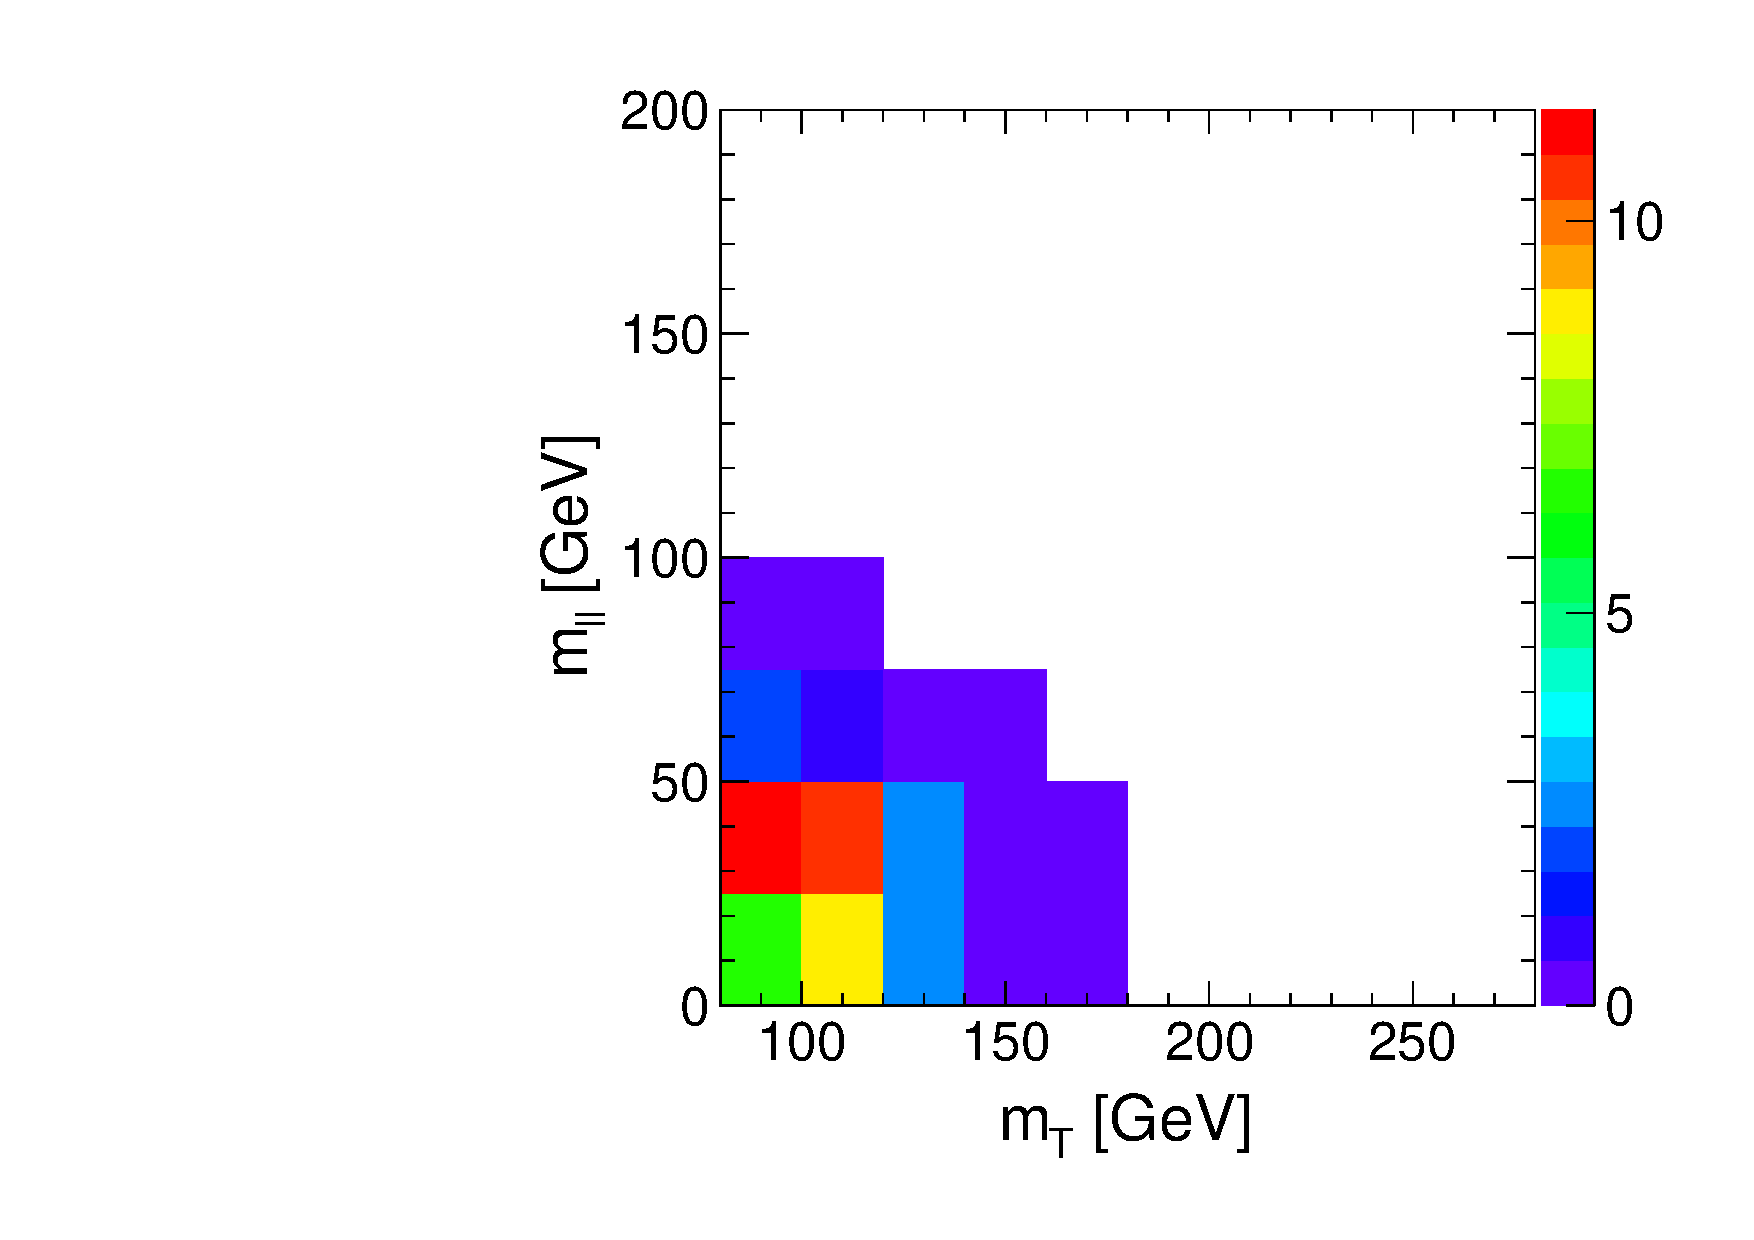
\includegraphics[width=.3\textwidth]{figures/mtvsmll_hww_120_0j.pdf}
}
\subfigure[mH(125)]{
\centering
\label{subfig:h125_0j}
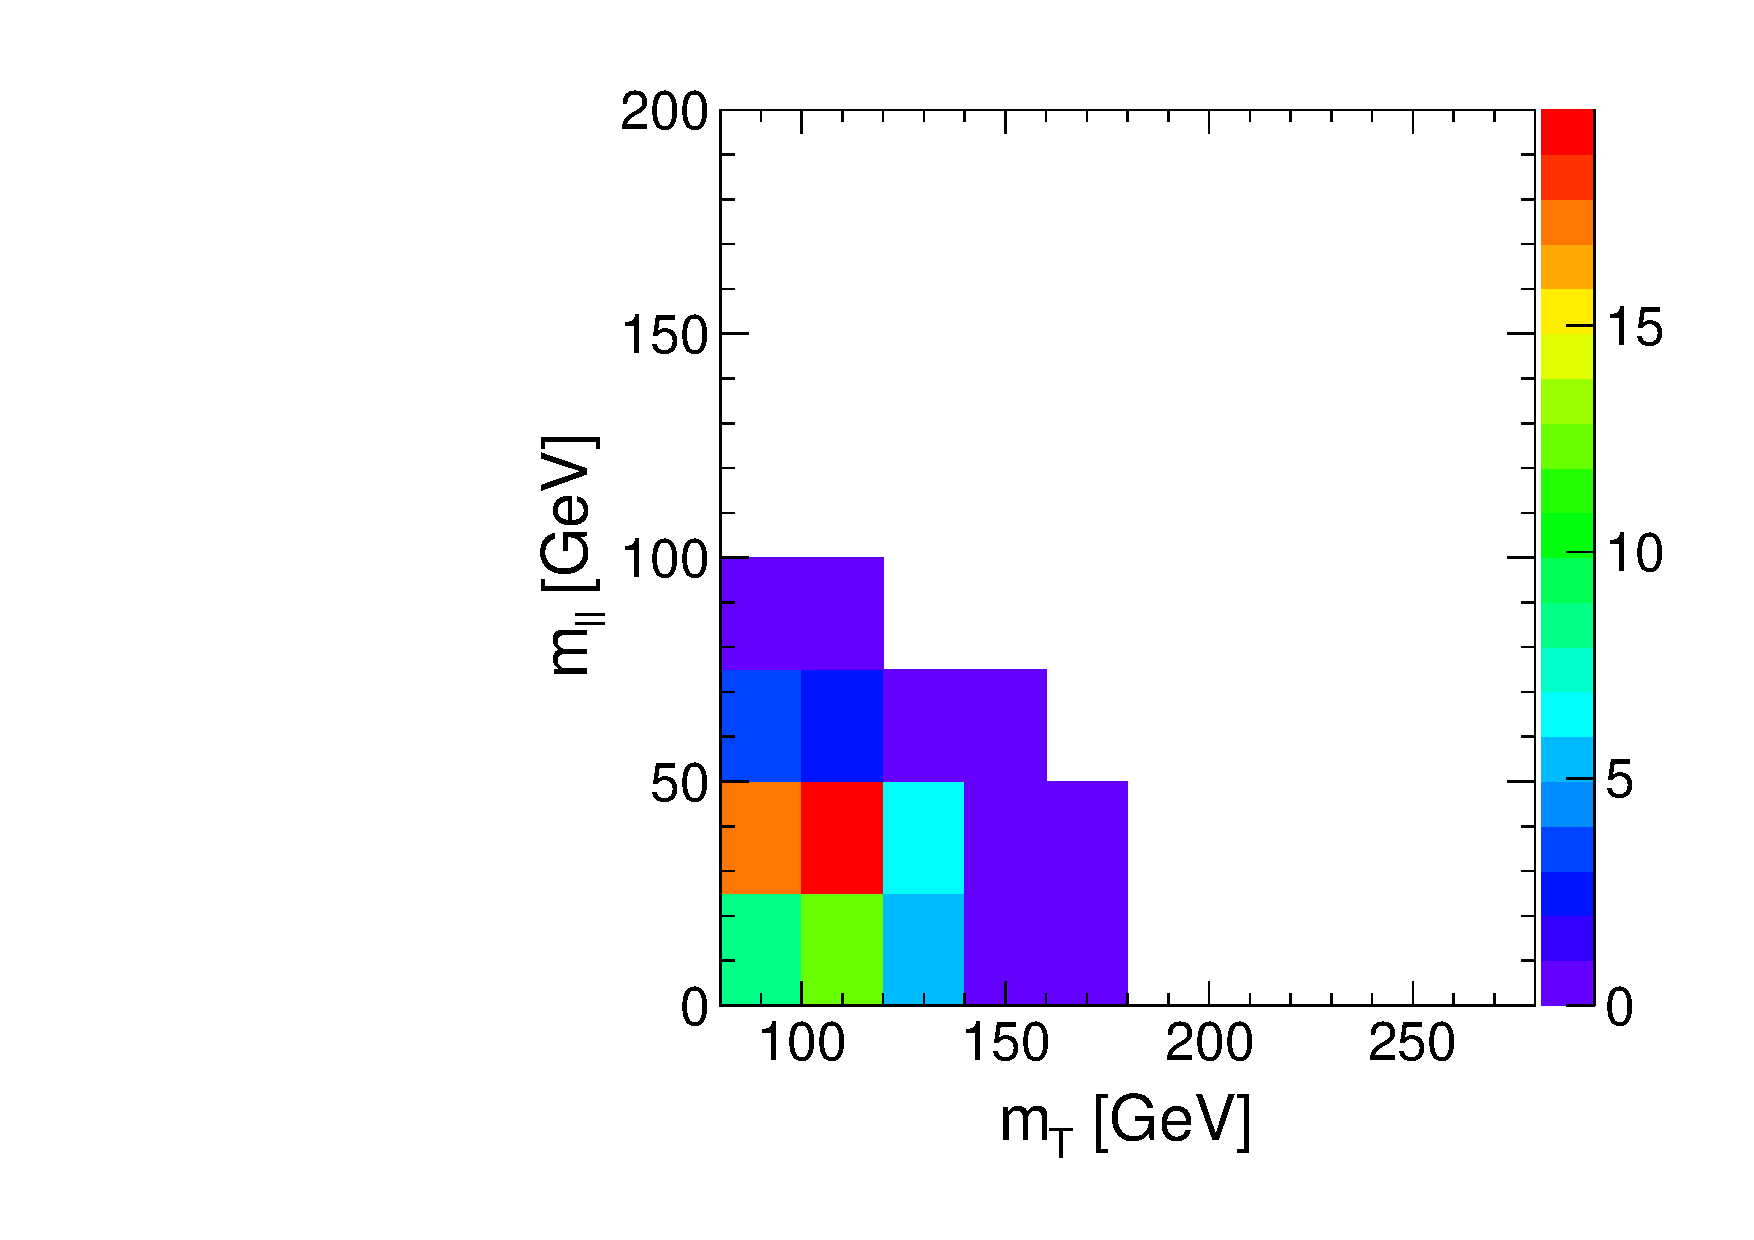
\includegraphics[width=.3\textwidth]{figures/mtvsmll_hww_125_0j.pdf}
} 
\subfigure[mH(130)]{
\centering
\label{subfig:h130_0j}
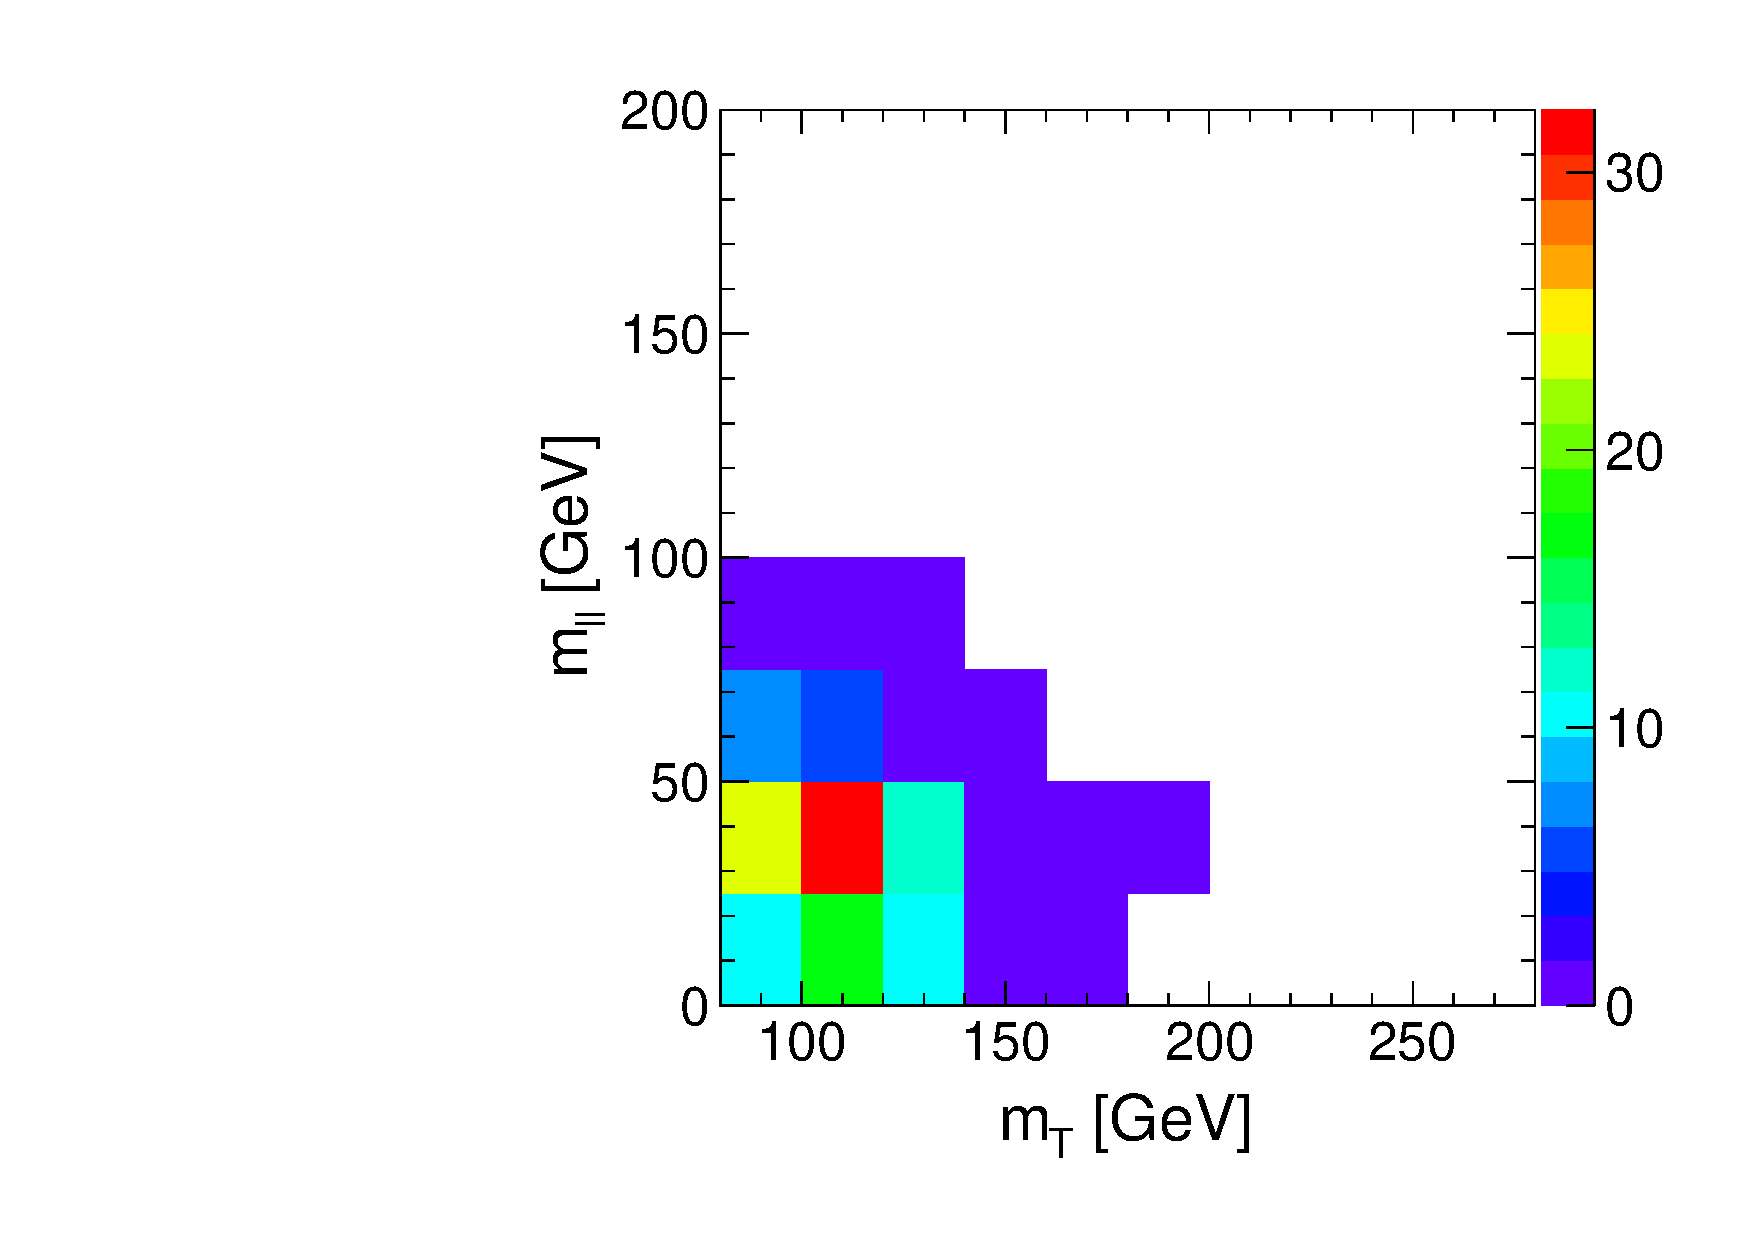
\includegraphics[width=.3\textwidth]{figures/mtvsmll_hww_130_0j.pdf}
}\\
\subfigure[mH(135)]{
\centering
\label{subfig:h135_0j}
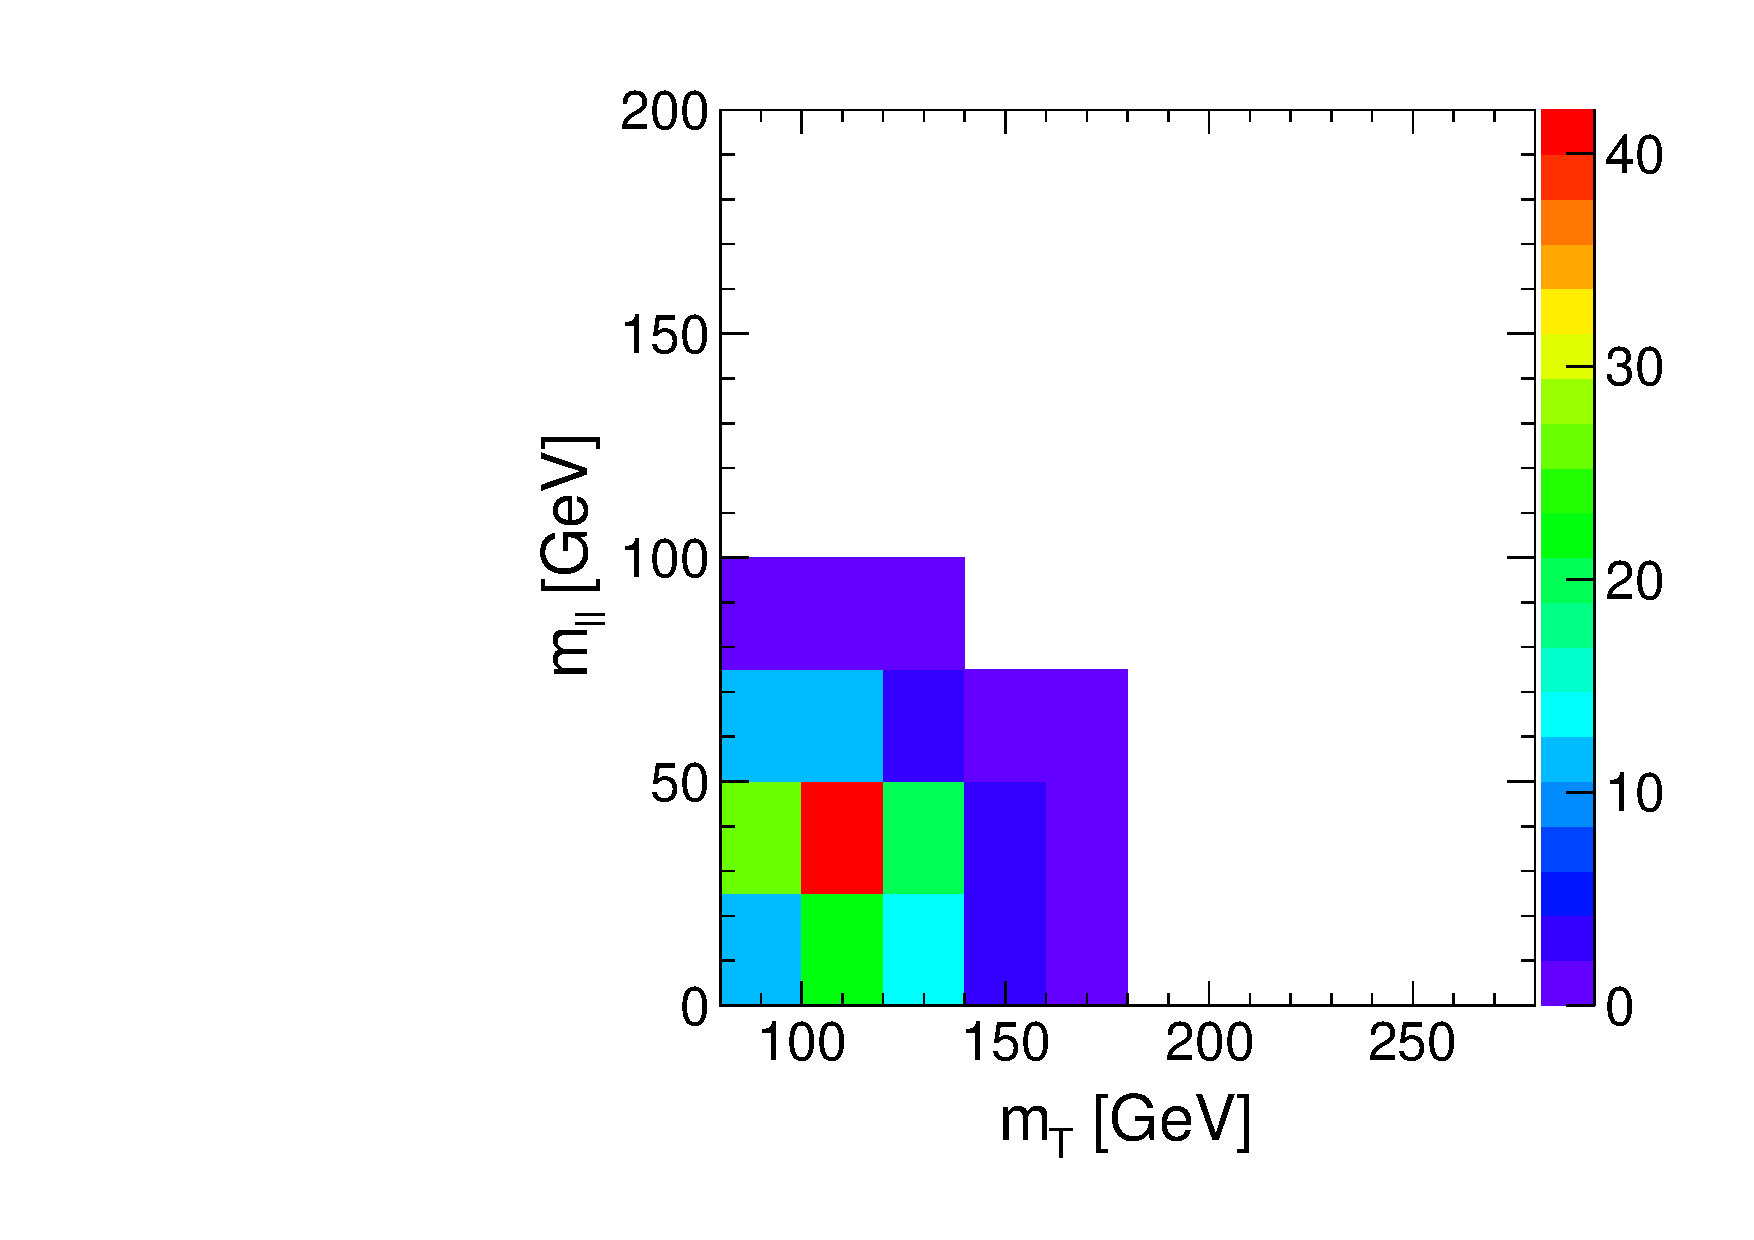
\includegraphics[width=.3\textwidth]{figures/mtvsmll_hww_135_0j.pdf}
}
\subfigure[mH(140)]{
\centering
\label{subfig:h140_0j}
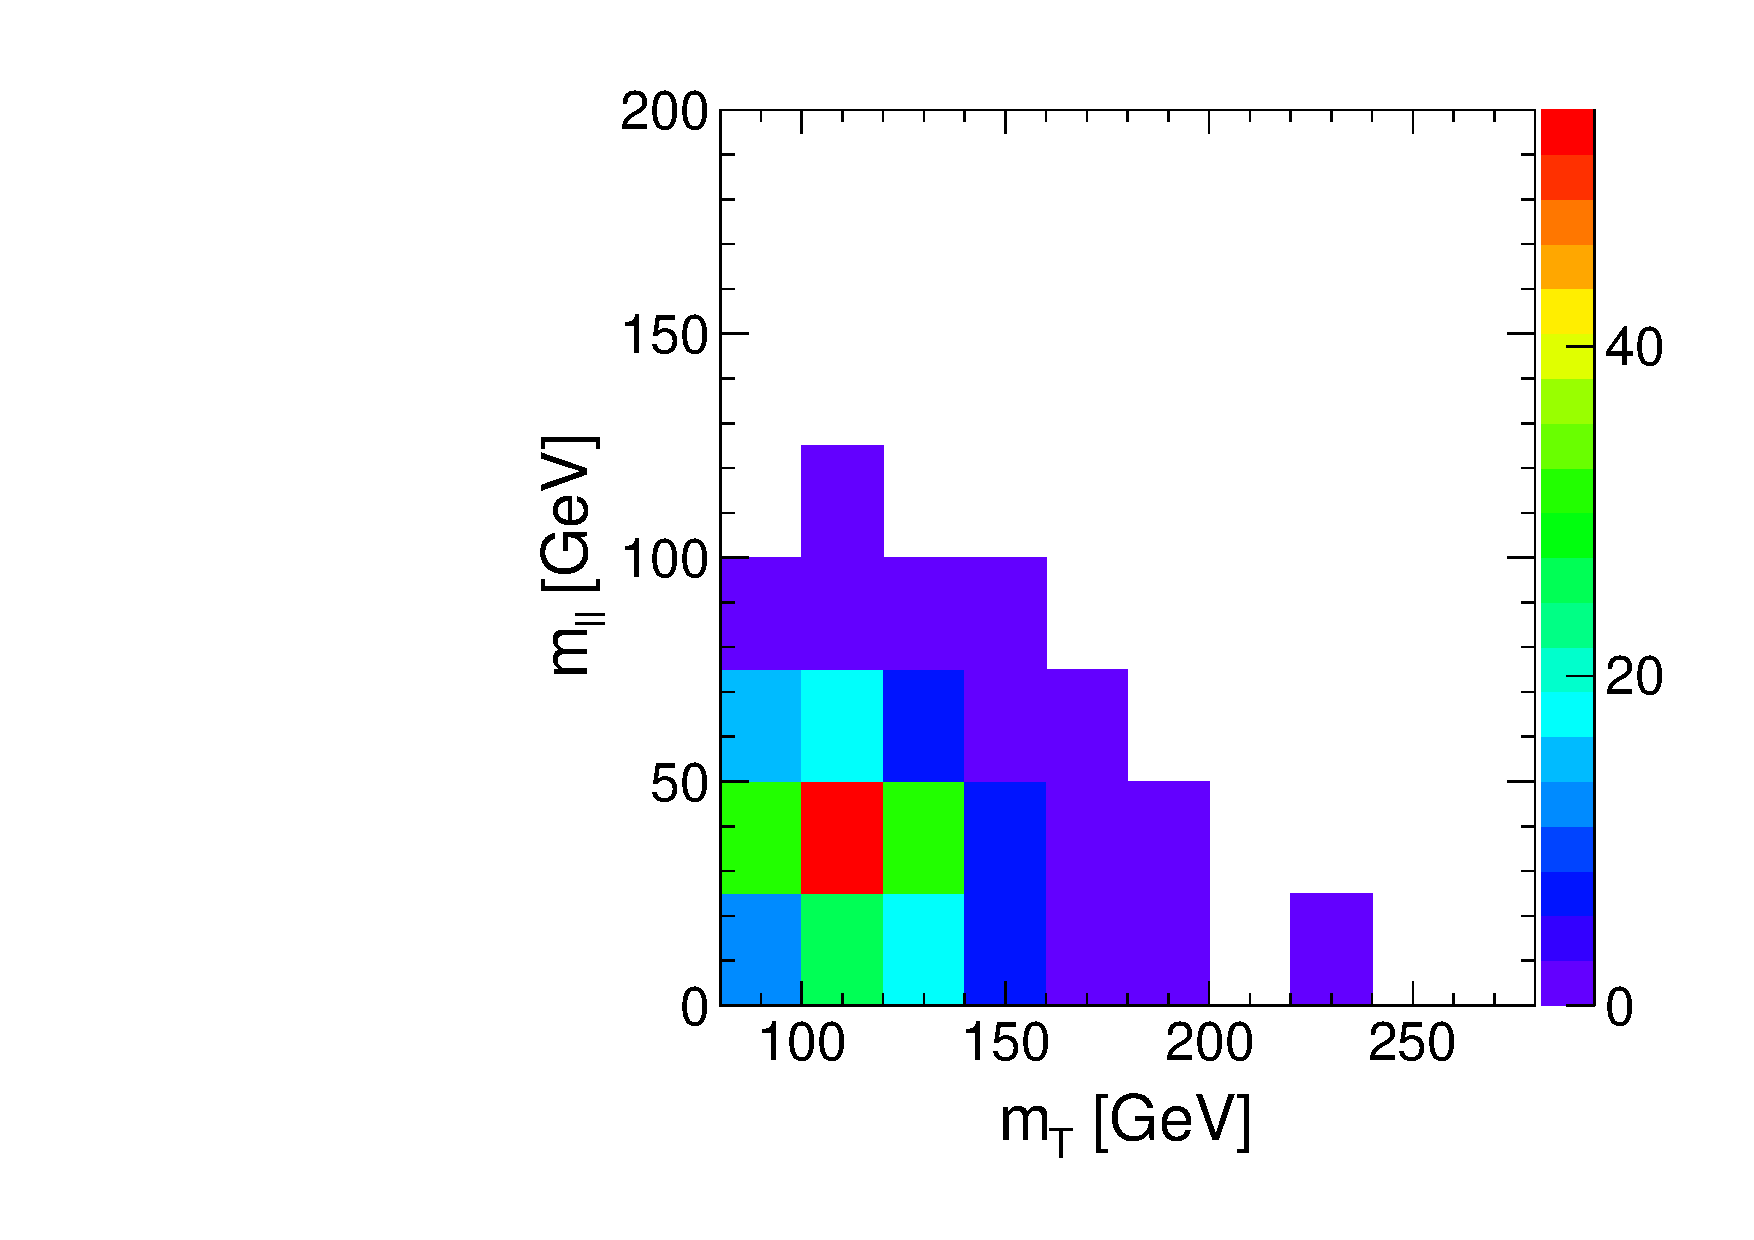
\includegraphics[width=.3\textwidth]{figures/mtvsmll_hww_140_0j.pdf}
}
\subfigure[mH(150)]{
\centering
\label{subfig:h150_0j}
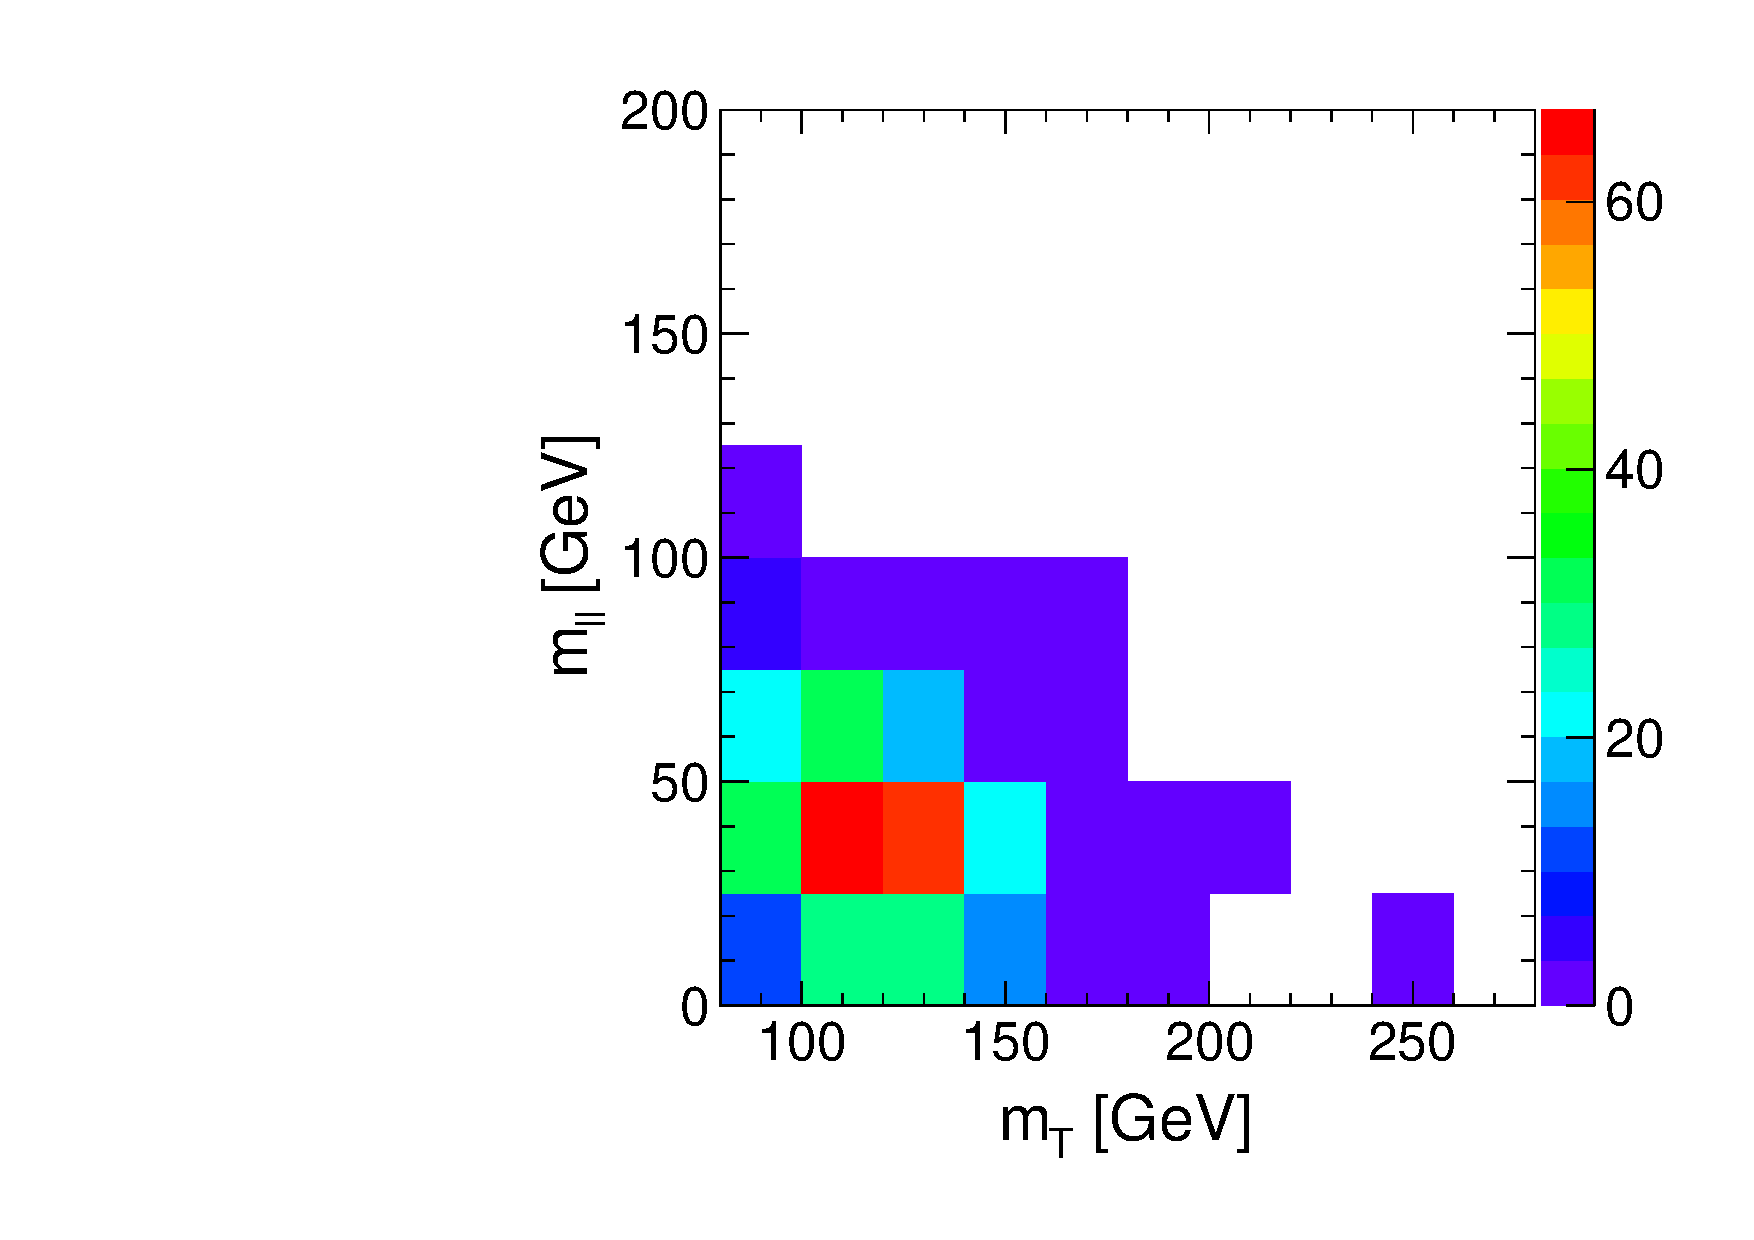
\includegraphics[width=.3\textwidth]{figures/mtvsmll_hww_150_0j.pdf}
} \\
\subfigure[mH(160)]{
\centering
\label{subfig:h160_0j}
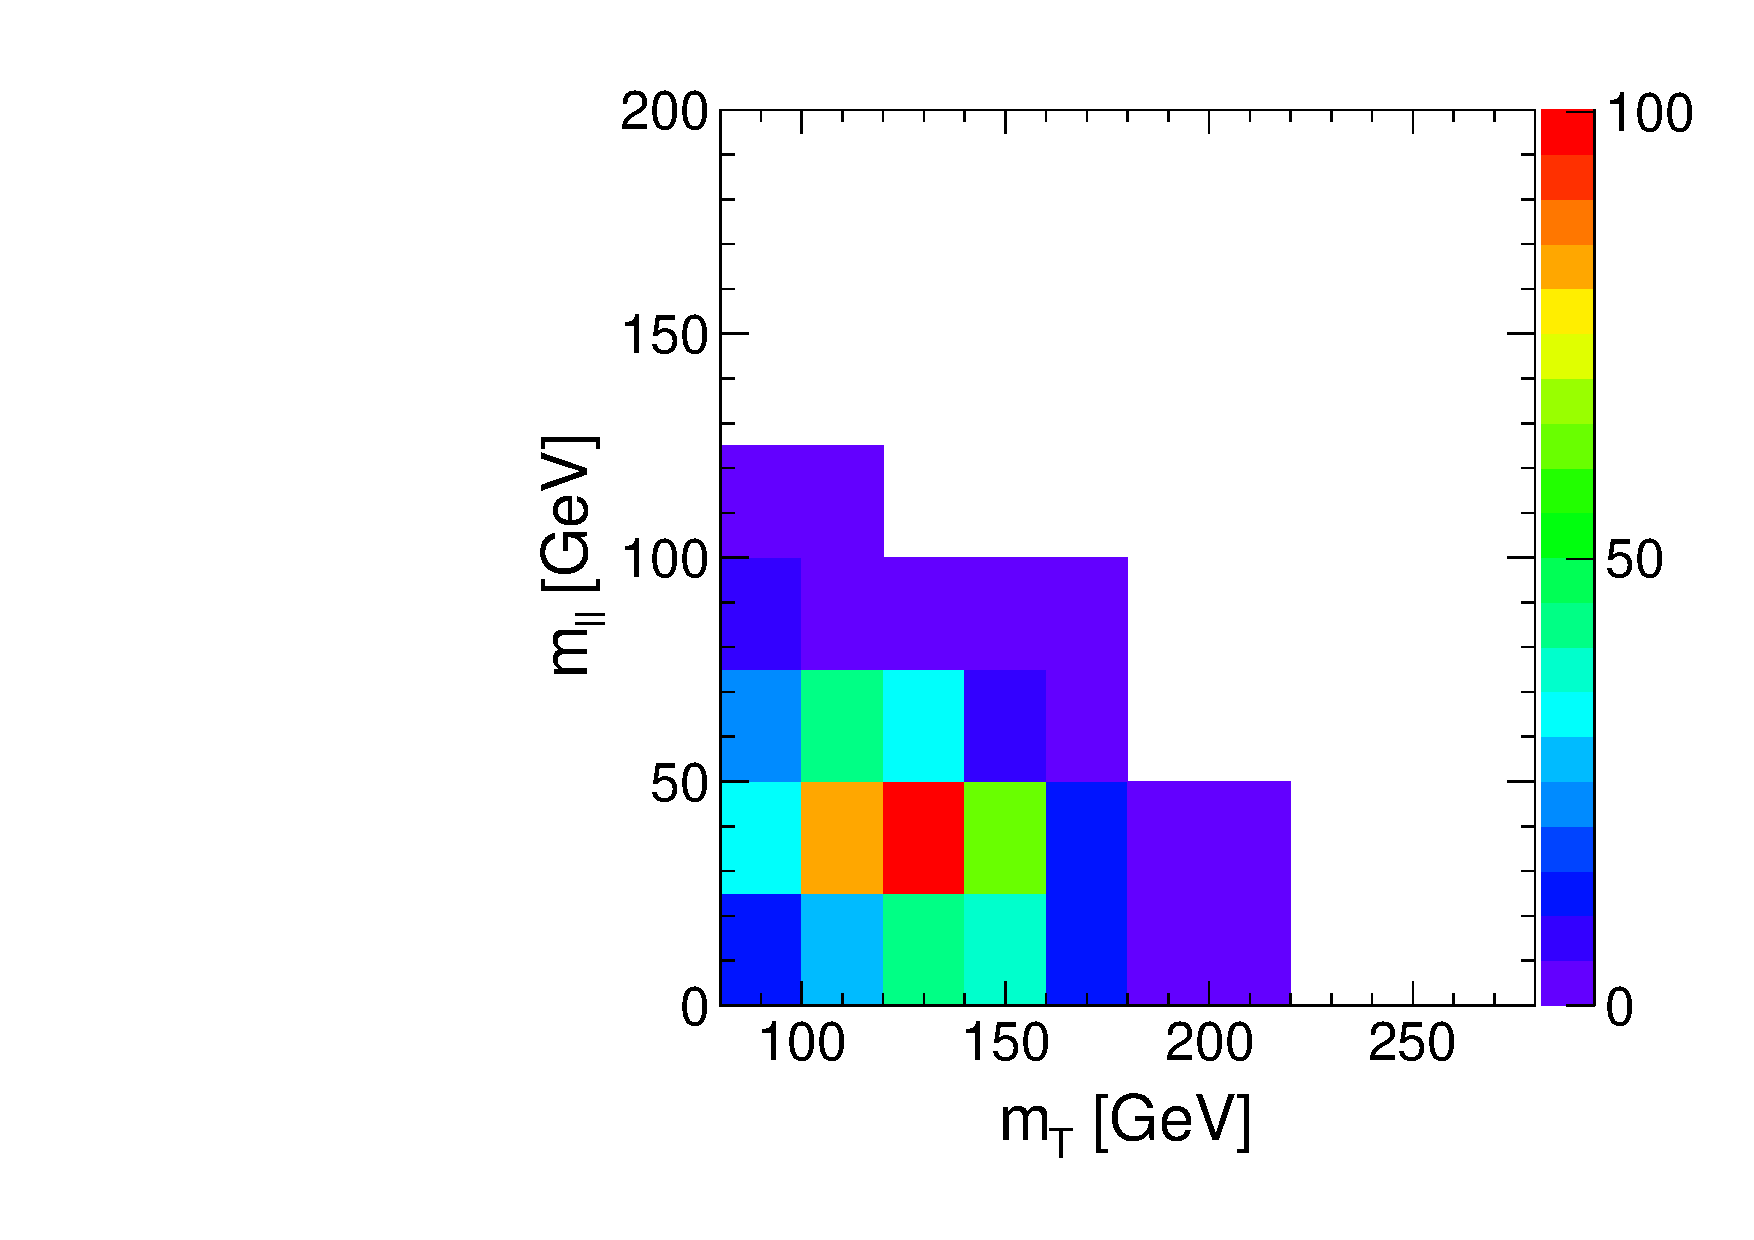
\includegraphics[width=.3\textwidth]{figures/mtvsmll_hww_160_0j.pdf}
}
\subfigure[mH(170)]{
\centering
\label{subfig:h170_0j}
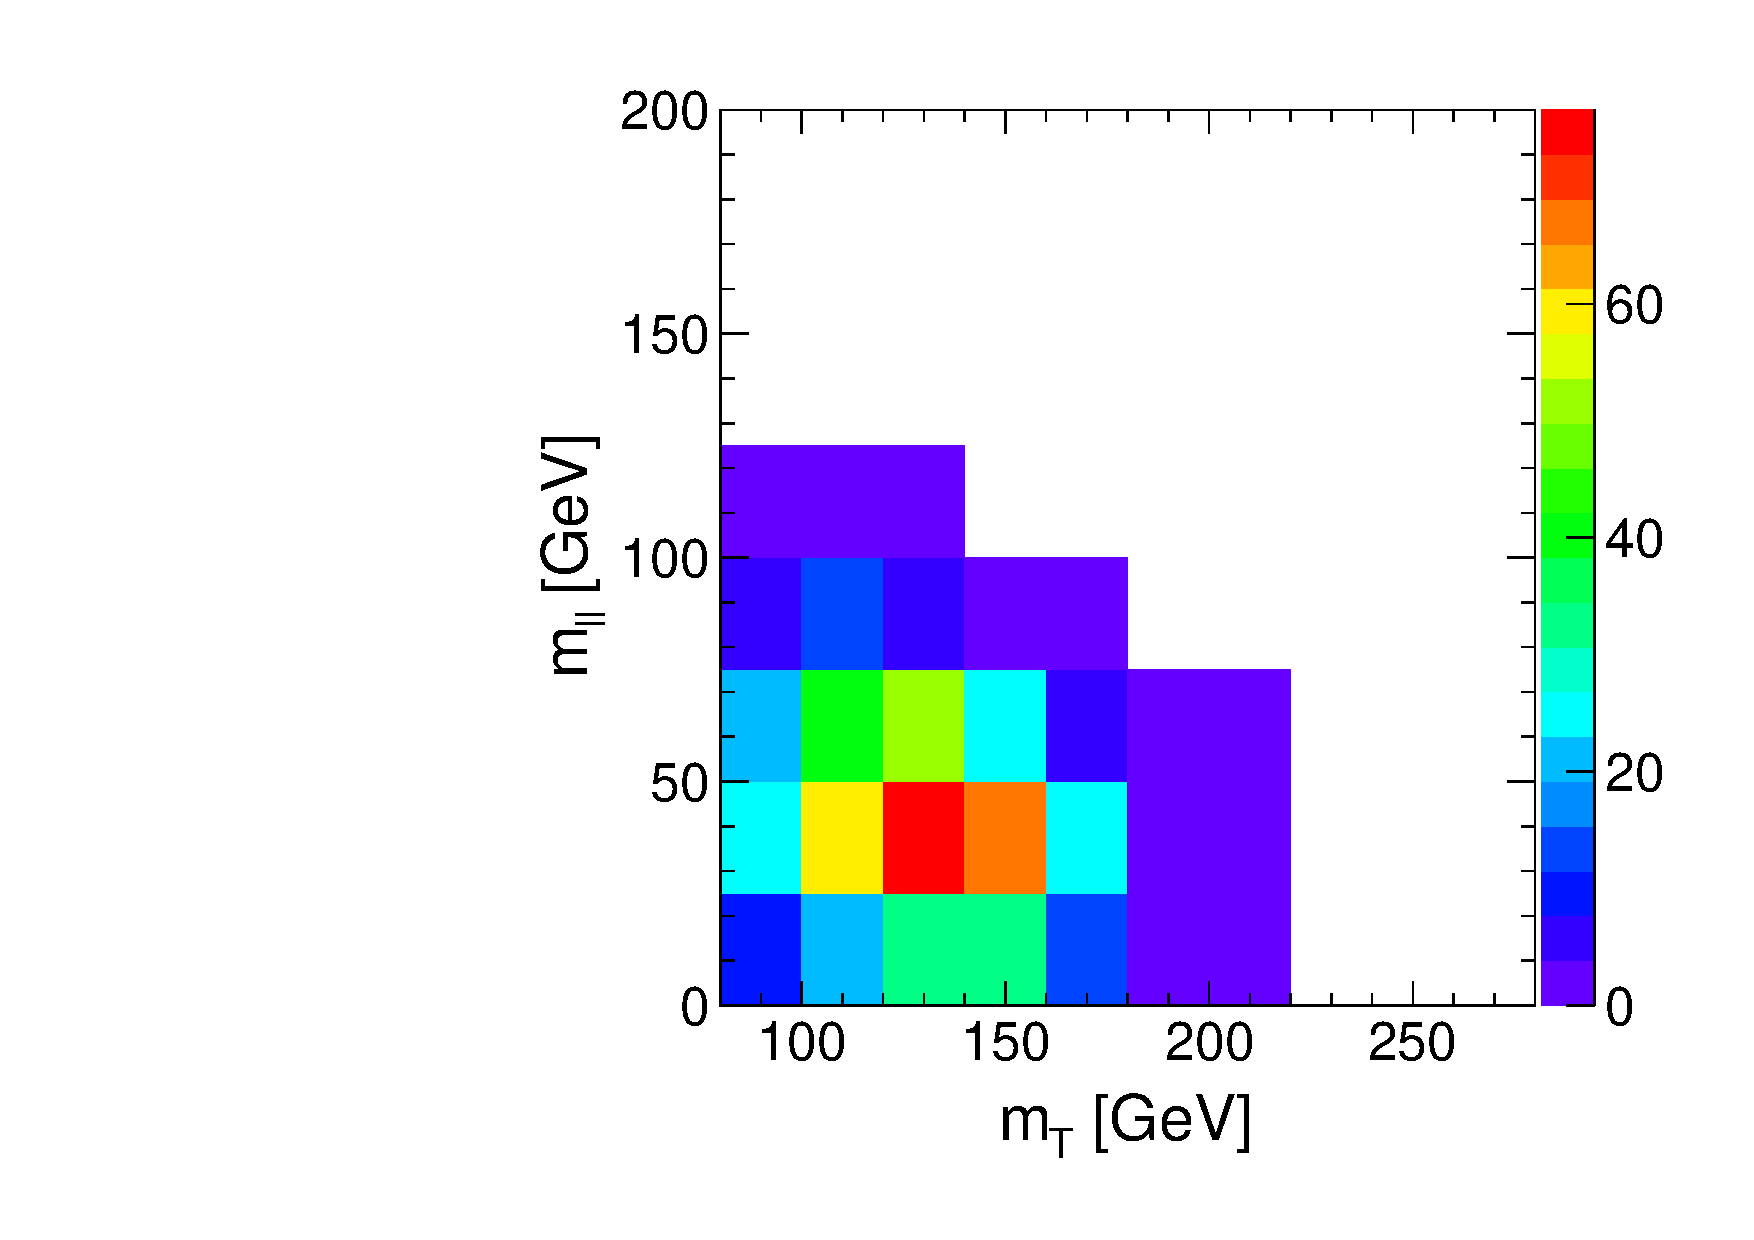
\includegraphics[width=.3\textwidth]{figures/mtvsmll_hww_170_0j.pdf}
} 
\subfigure[mH(180)]{
\centering
\label{subfig:h180_0j}
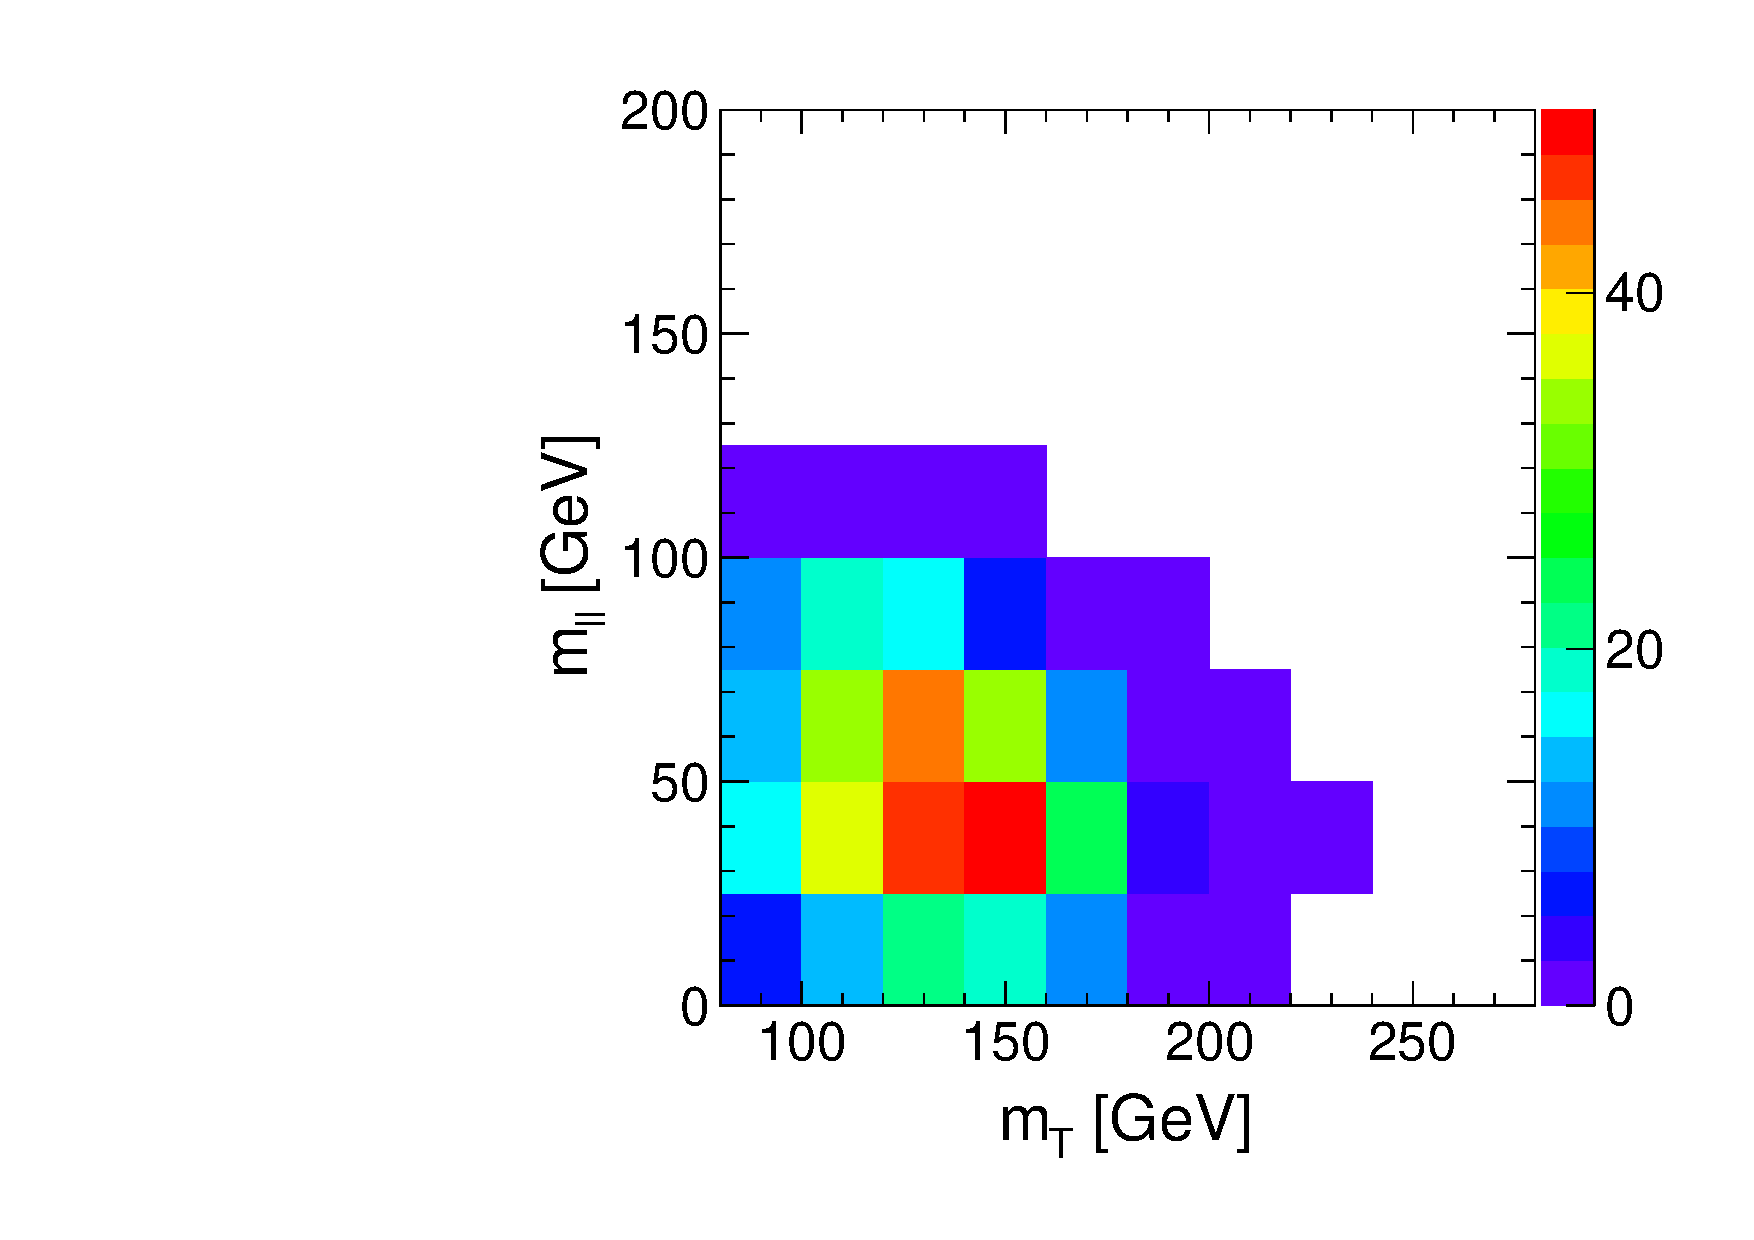
\includegraphics[width=.3\textwidth]{figures/mtvsmll_hww_180_0j.pdf}
} \\
\subfigure[mH(190)]{
\centering
\label{subfig:h190_0j}
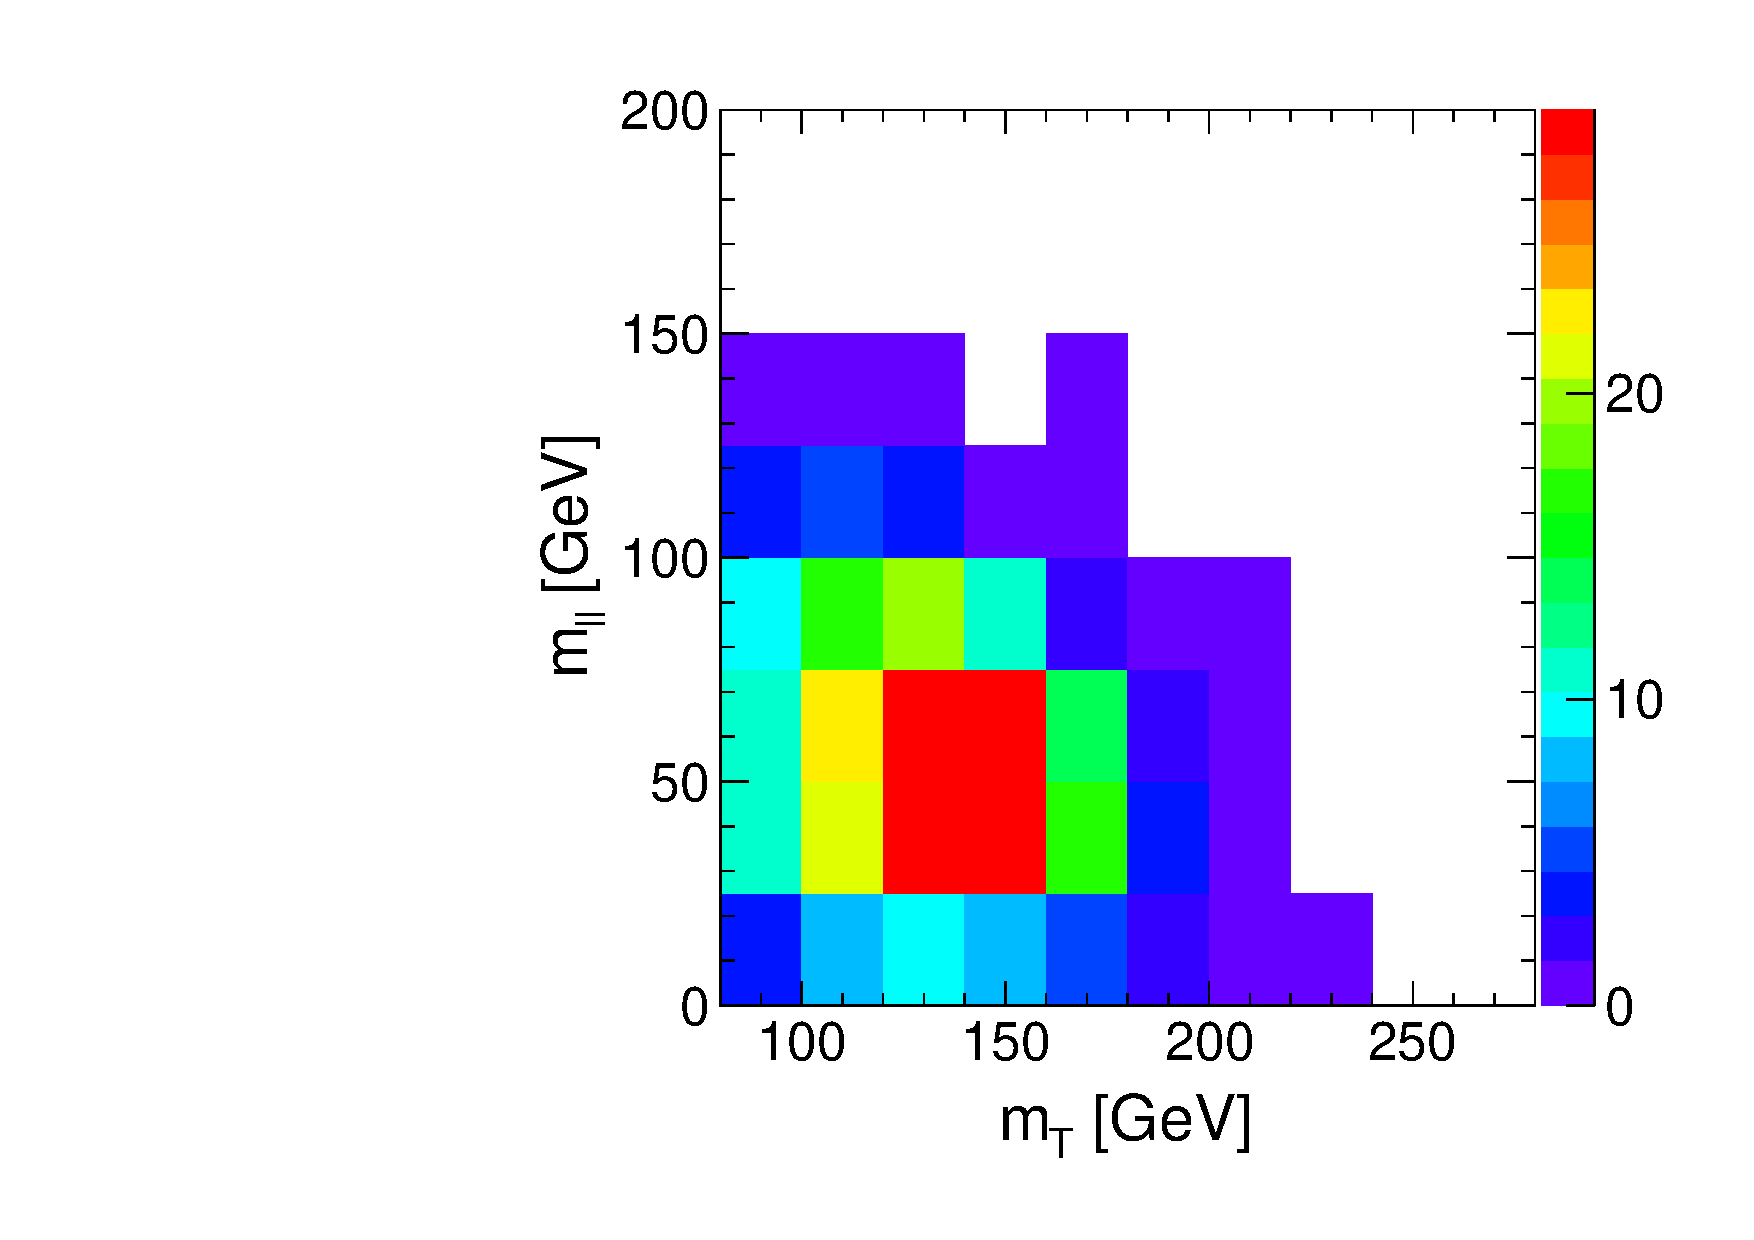
\includegraphics[width=.3\textwidth]{figures/mtvsmll_hww_190_0j.pdf}
}
\subfigure[mH(200)]{
\centering
\label{subfig:h200_0j}
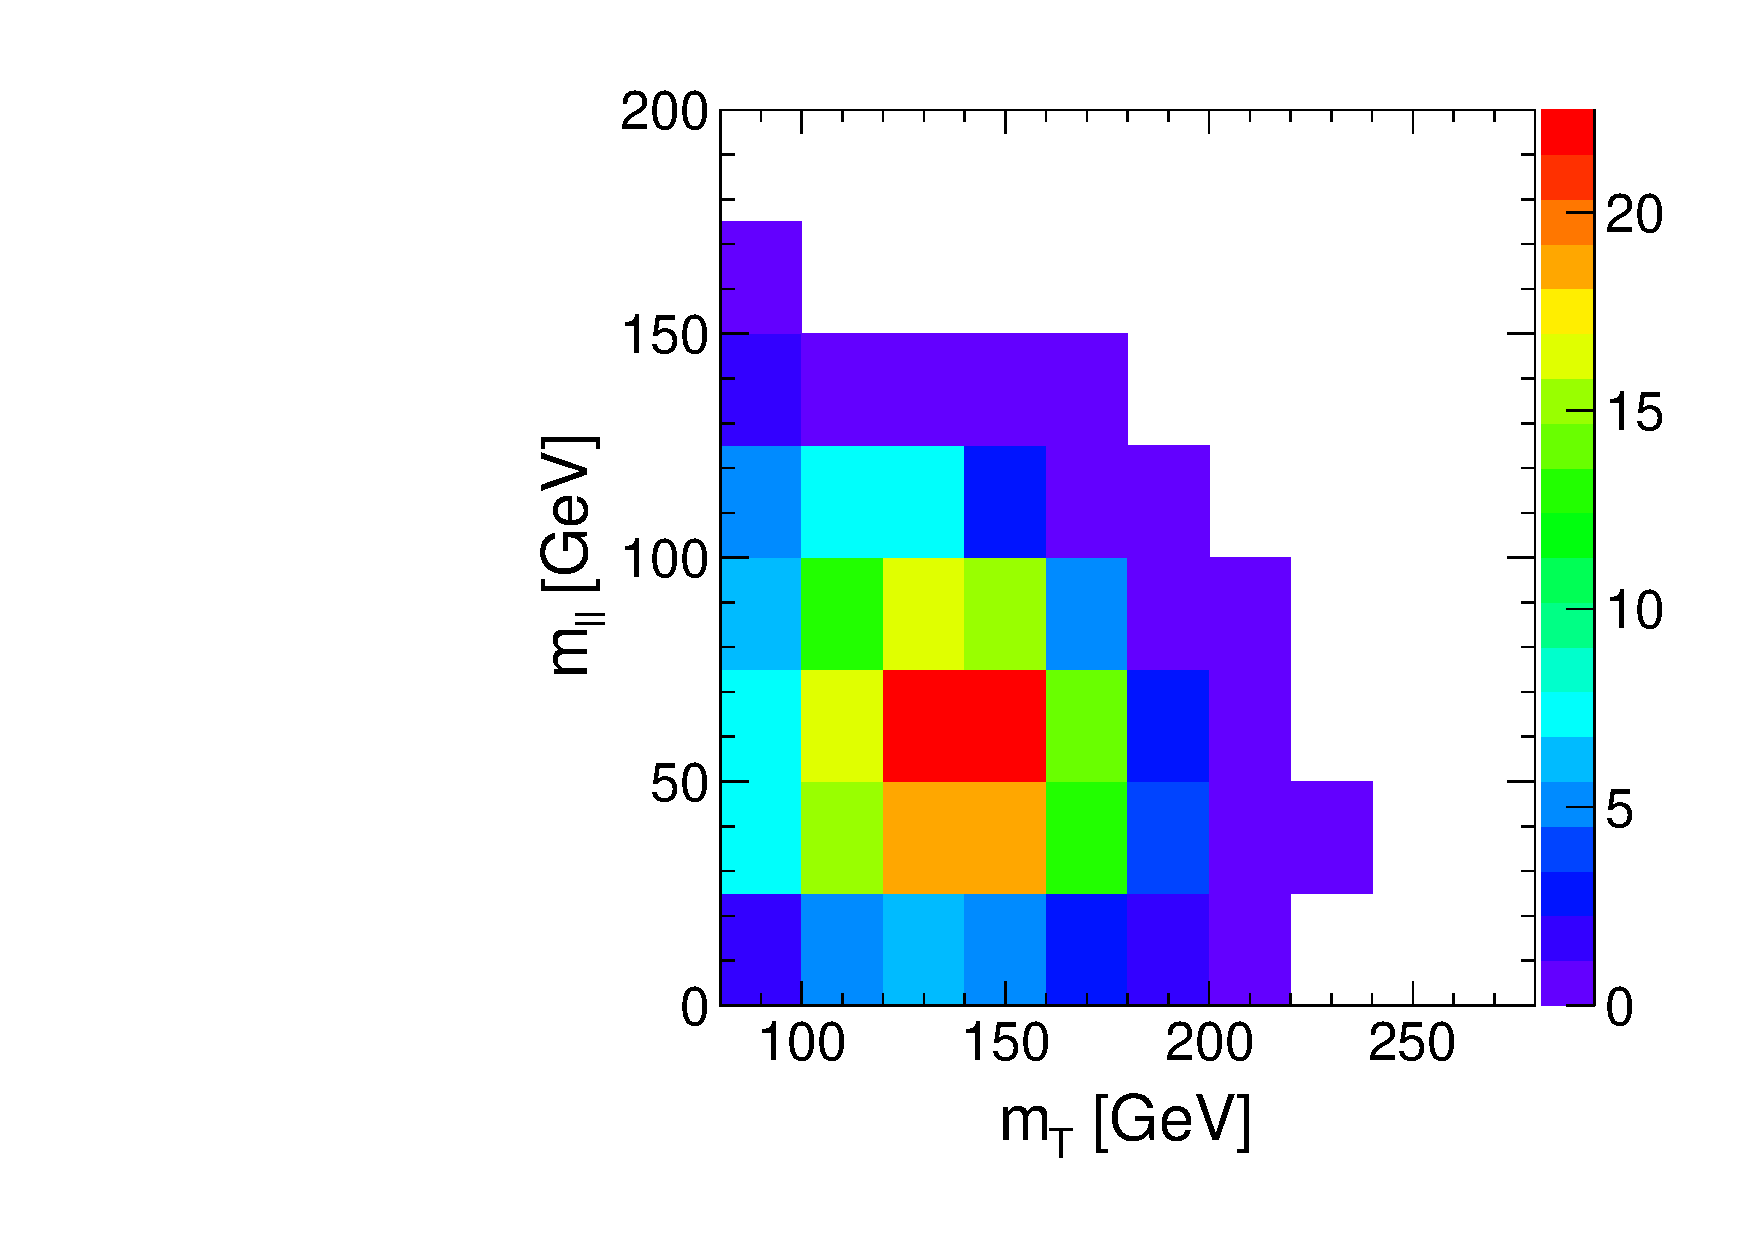
\includegraphics[width=.3\textwidth]{figures/mtvsmll_hww_200_0j.pdf}
} 
\subfigure[mH(250)]{
\centering
\label{subfig:h250_0j}
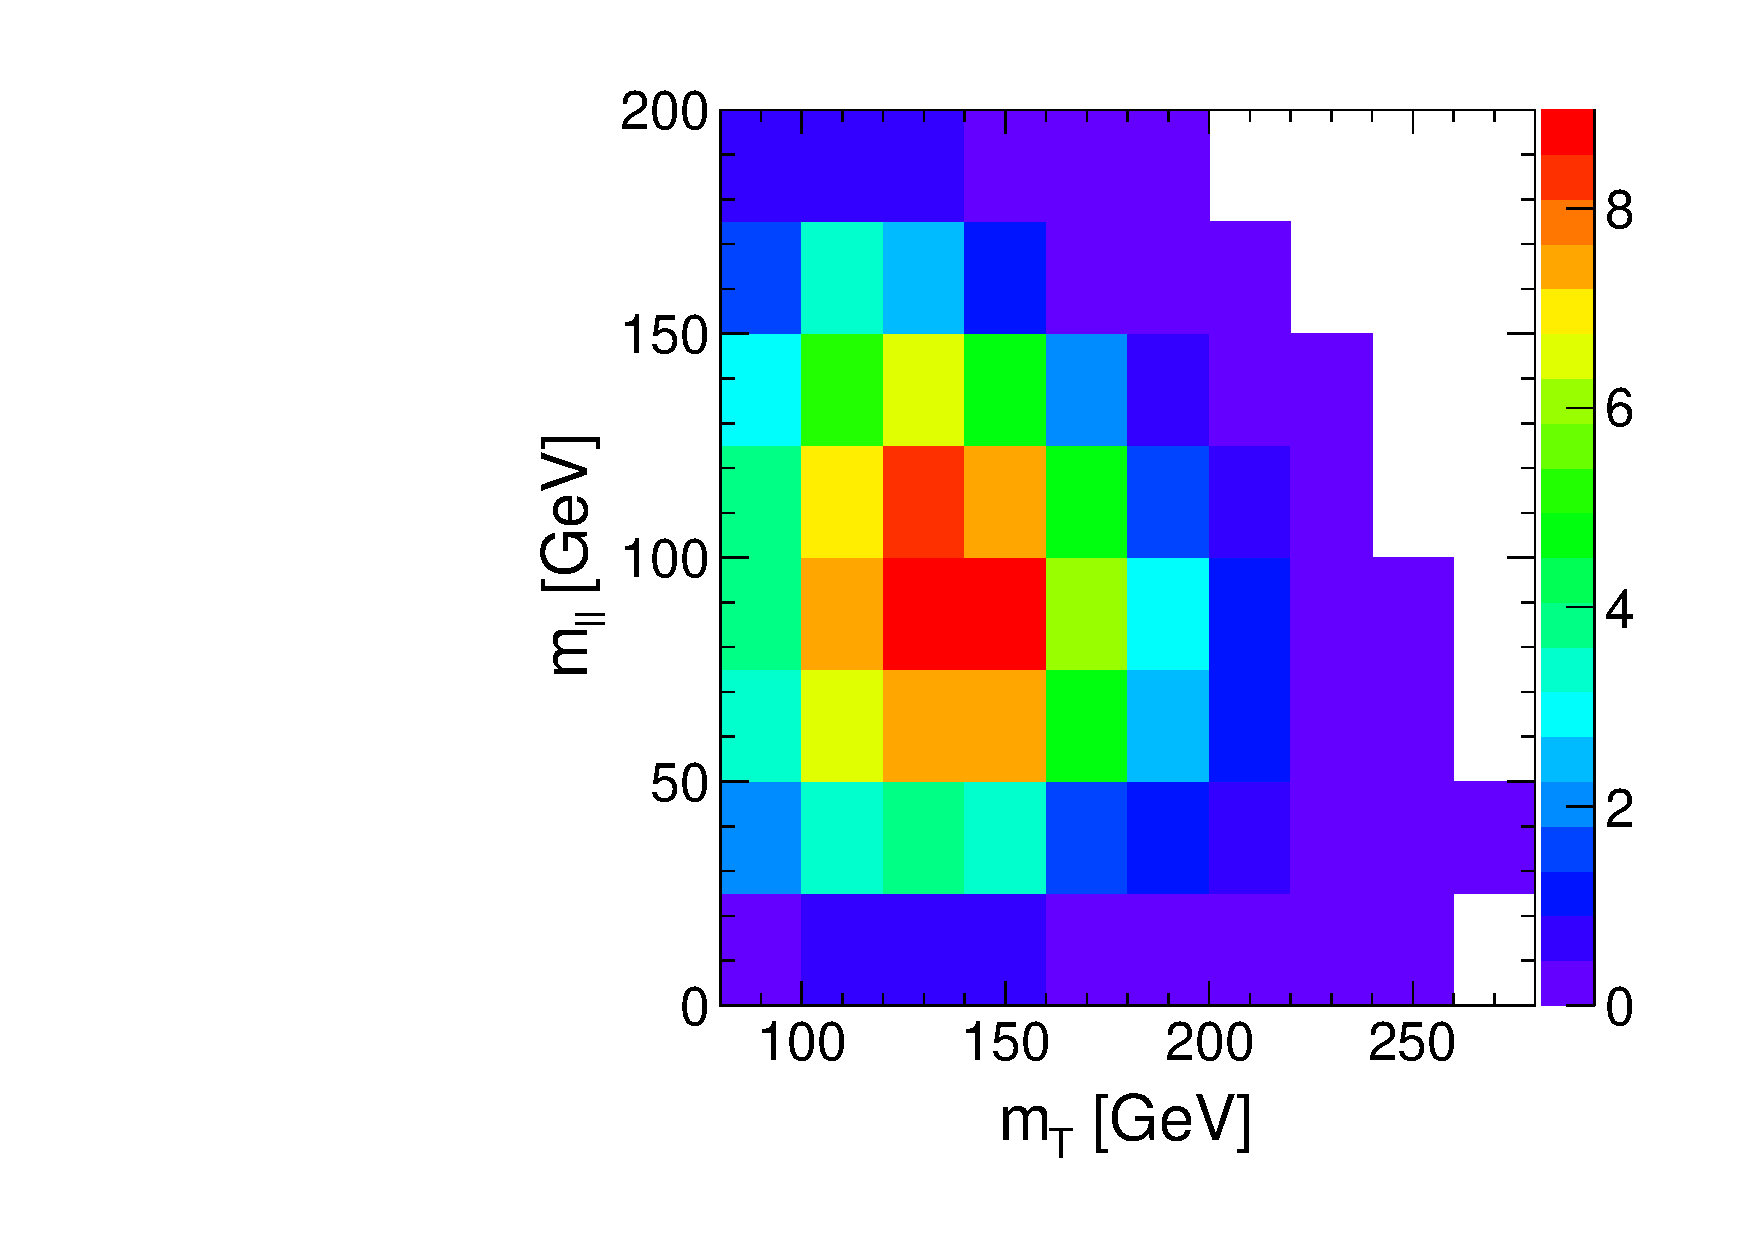
\includegraphics[width=.3\textwidth]{figures/mtvsmll_hww_250_0j.pdf}
} \\
\caption{ The 2D ($m_{ll}, m_T$) templates for the $gg\to H\to WW$ in the 0-Jet bin with $m_H<300$ GeV. }
\label{fig:hww2d_lowmass_0j}
\end{figure}
%%%%%%%%%%%%%%%%%%%%%%%%%%%%%%%


%%%%%%%%%%%%%%%%%%%%%%%%%%%%%%%
\begin{figure}[!hbtp]
\centering
\subfigure[$qq\to WW$]{
\centering
\label{subfig:qqww_0j}
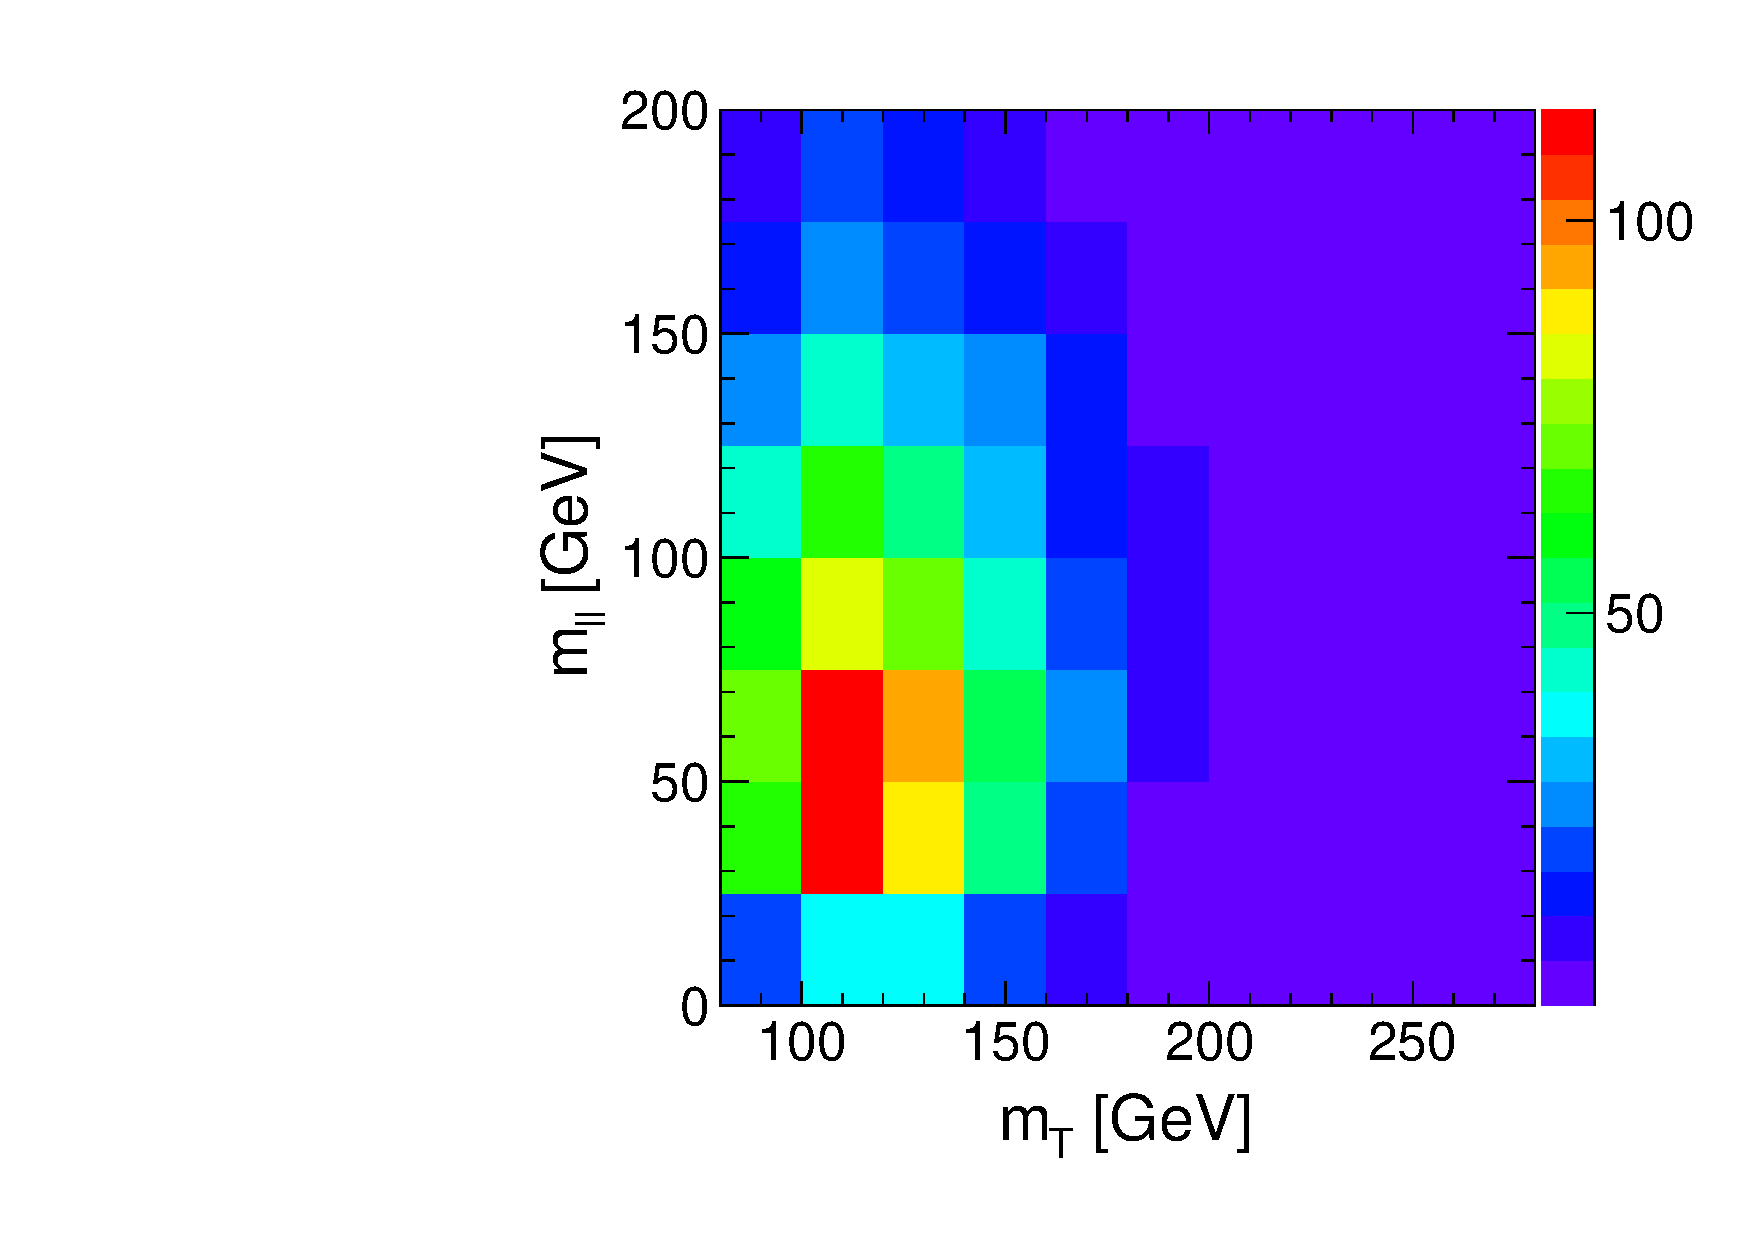
\includegraphics[width=.3\textwidth]{figures/mtvsmll_qqWW_lowmass_0j.pdf}
}
\subfigure[Top]{
\centering
\label{subfig:top_0j}
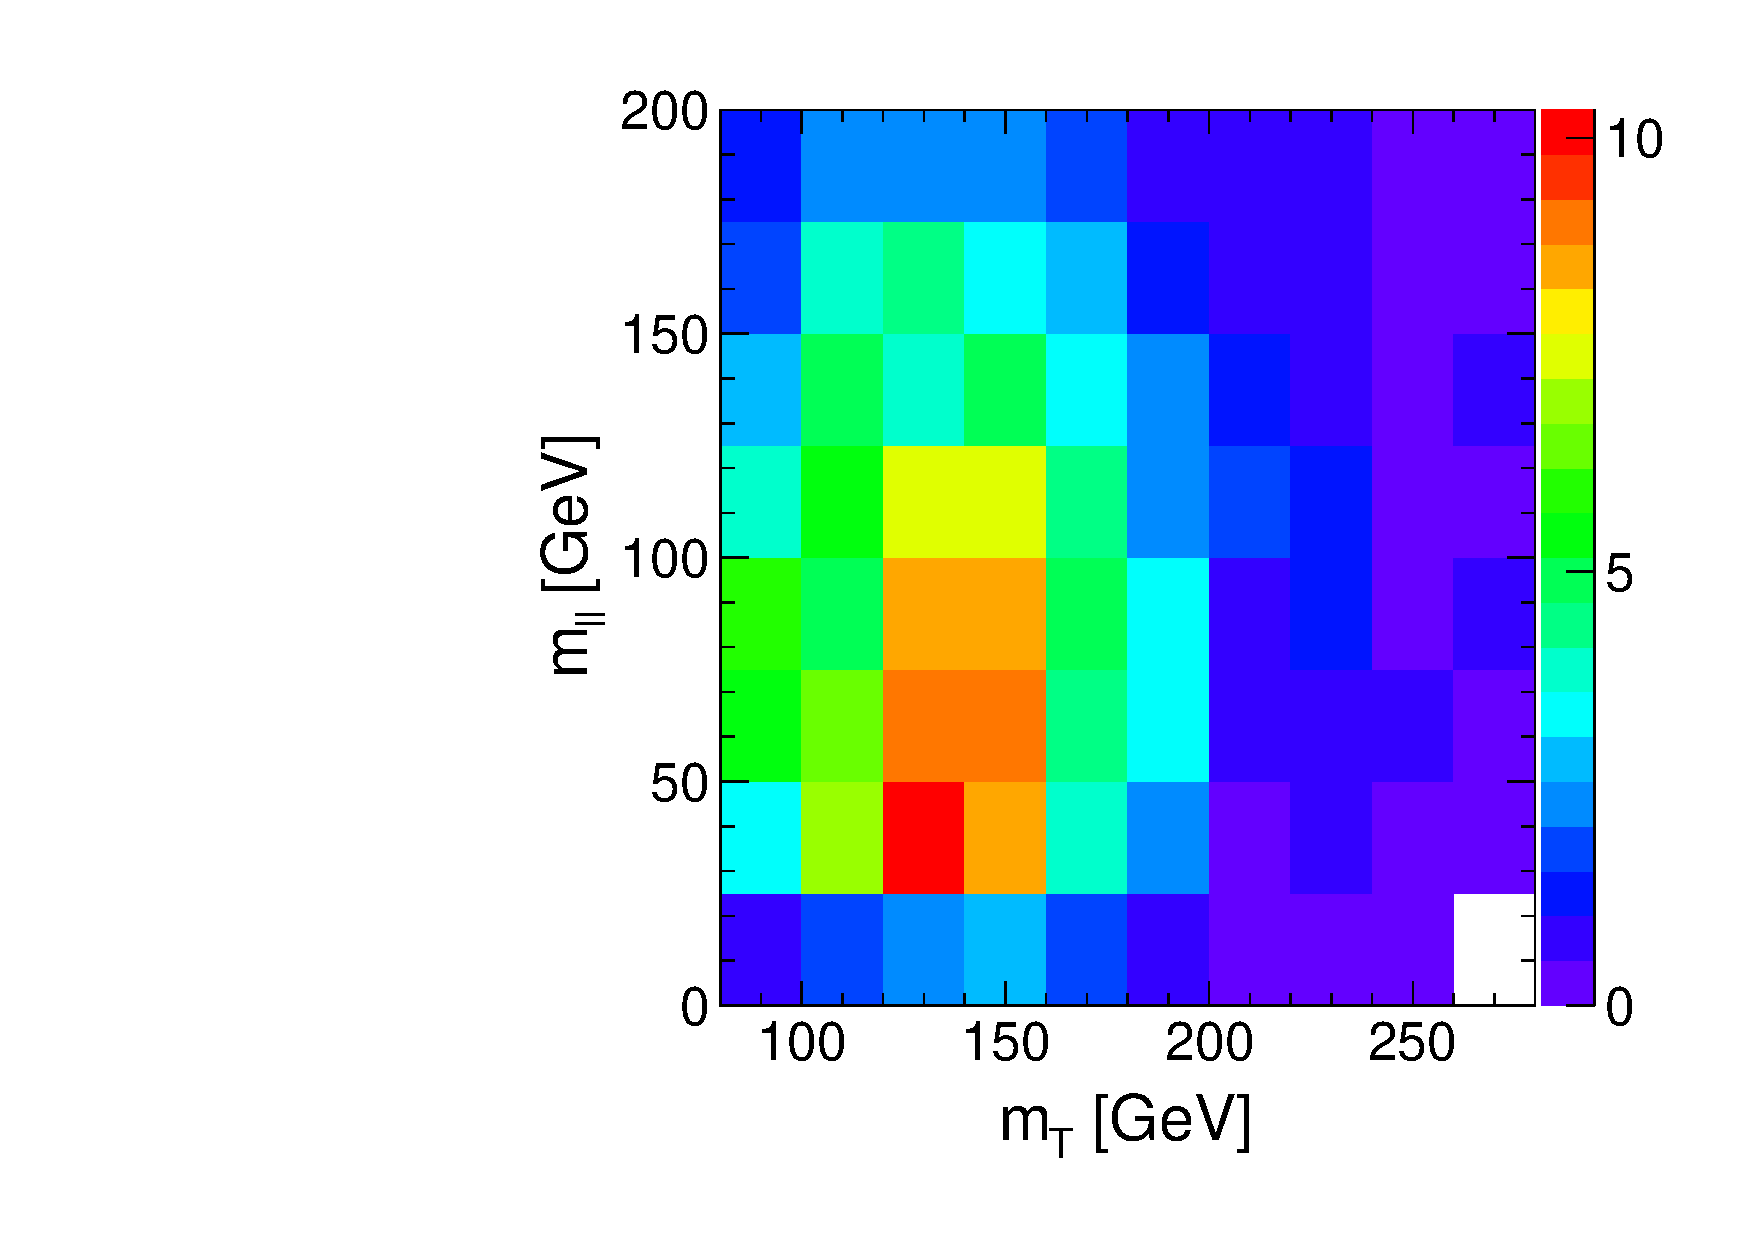
\includegraphics[width=.3\textwidth]{figures/mtvsmll_Top_lowmass_0j.pdf}
} \\ 
\subfigure[Wjets]{
\centering
\label{subfig:wjets_0j}
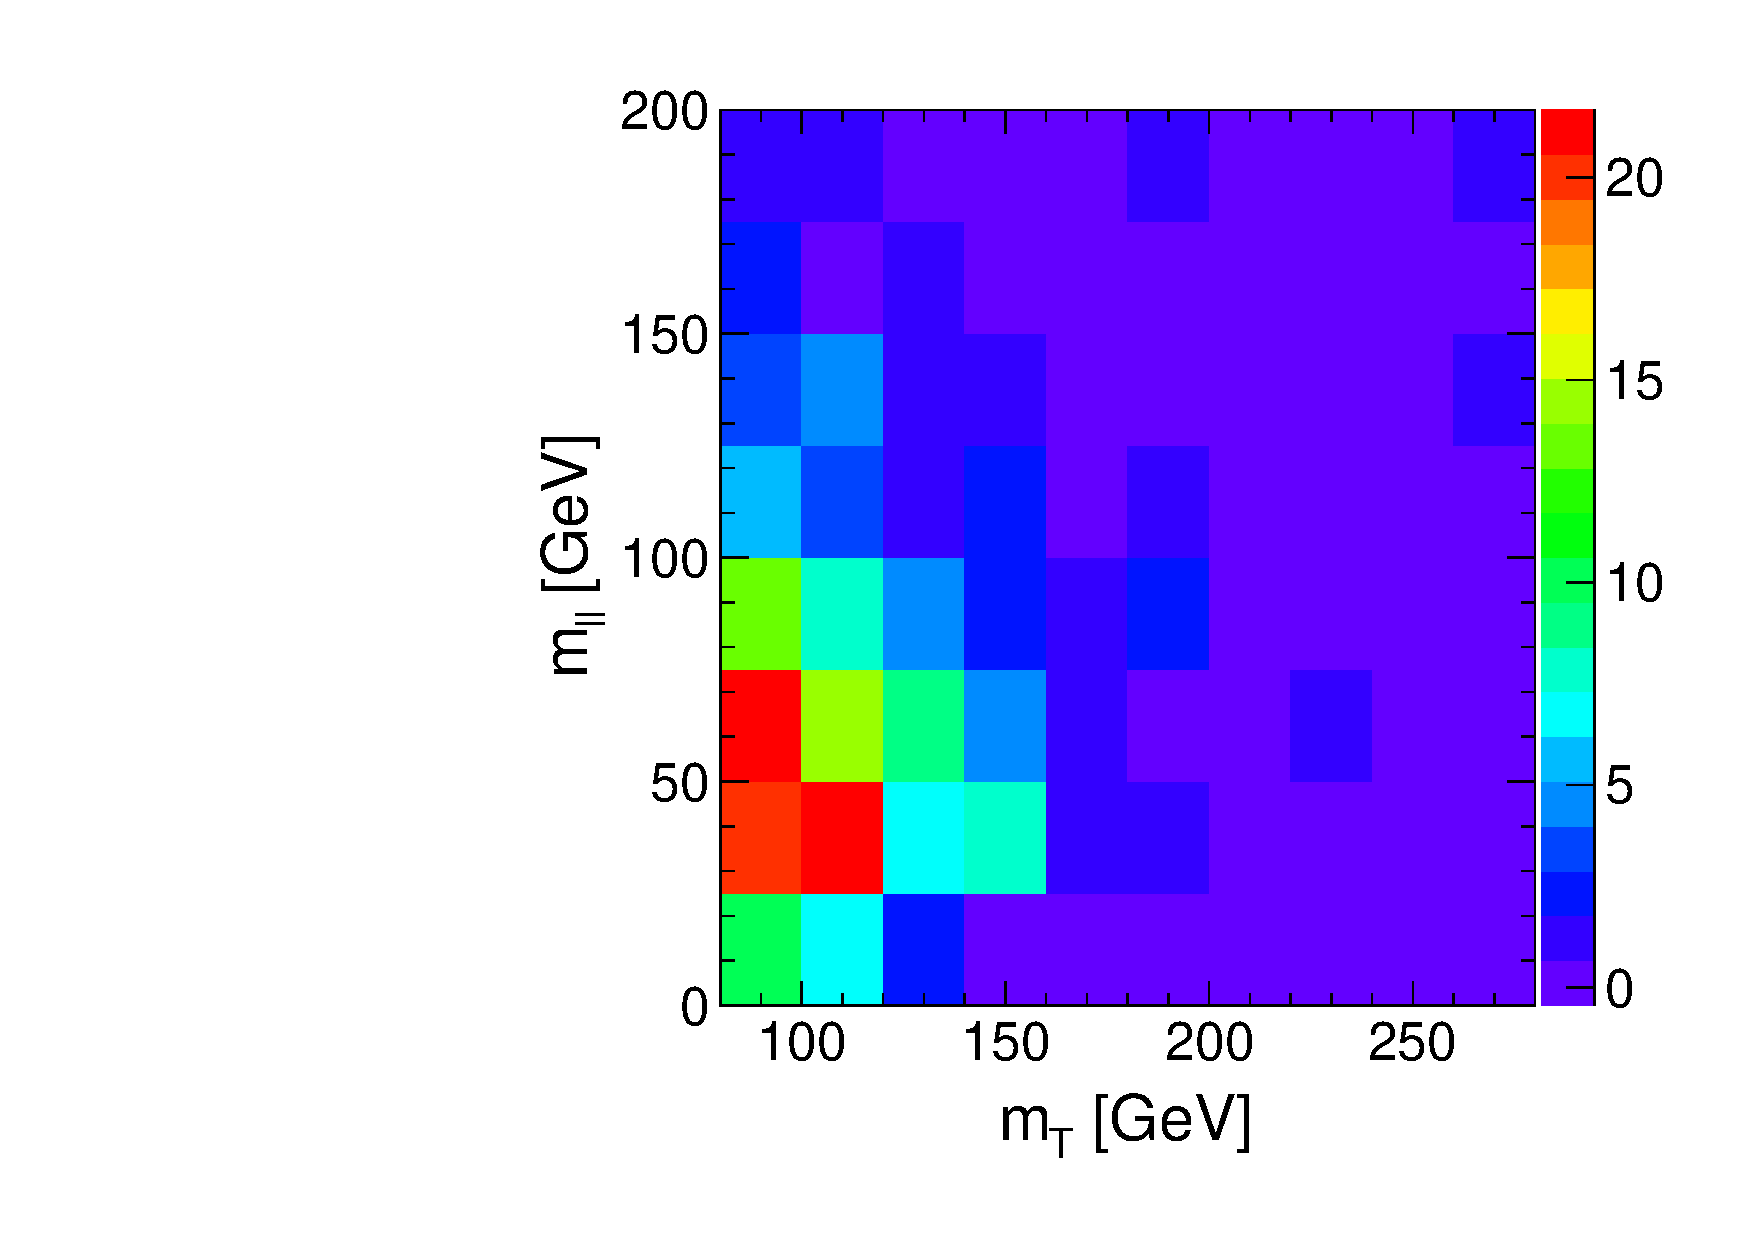
\includegraphics[width=.3\textwidth]{figures/mtvsmll_Wjets_lowmass_0j.pdf}
}
\subfigure[$W\gamma$]{
\centering
\label{subfig:wgamma_0j}
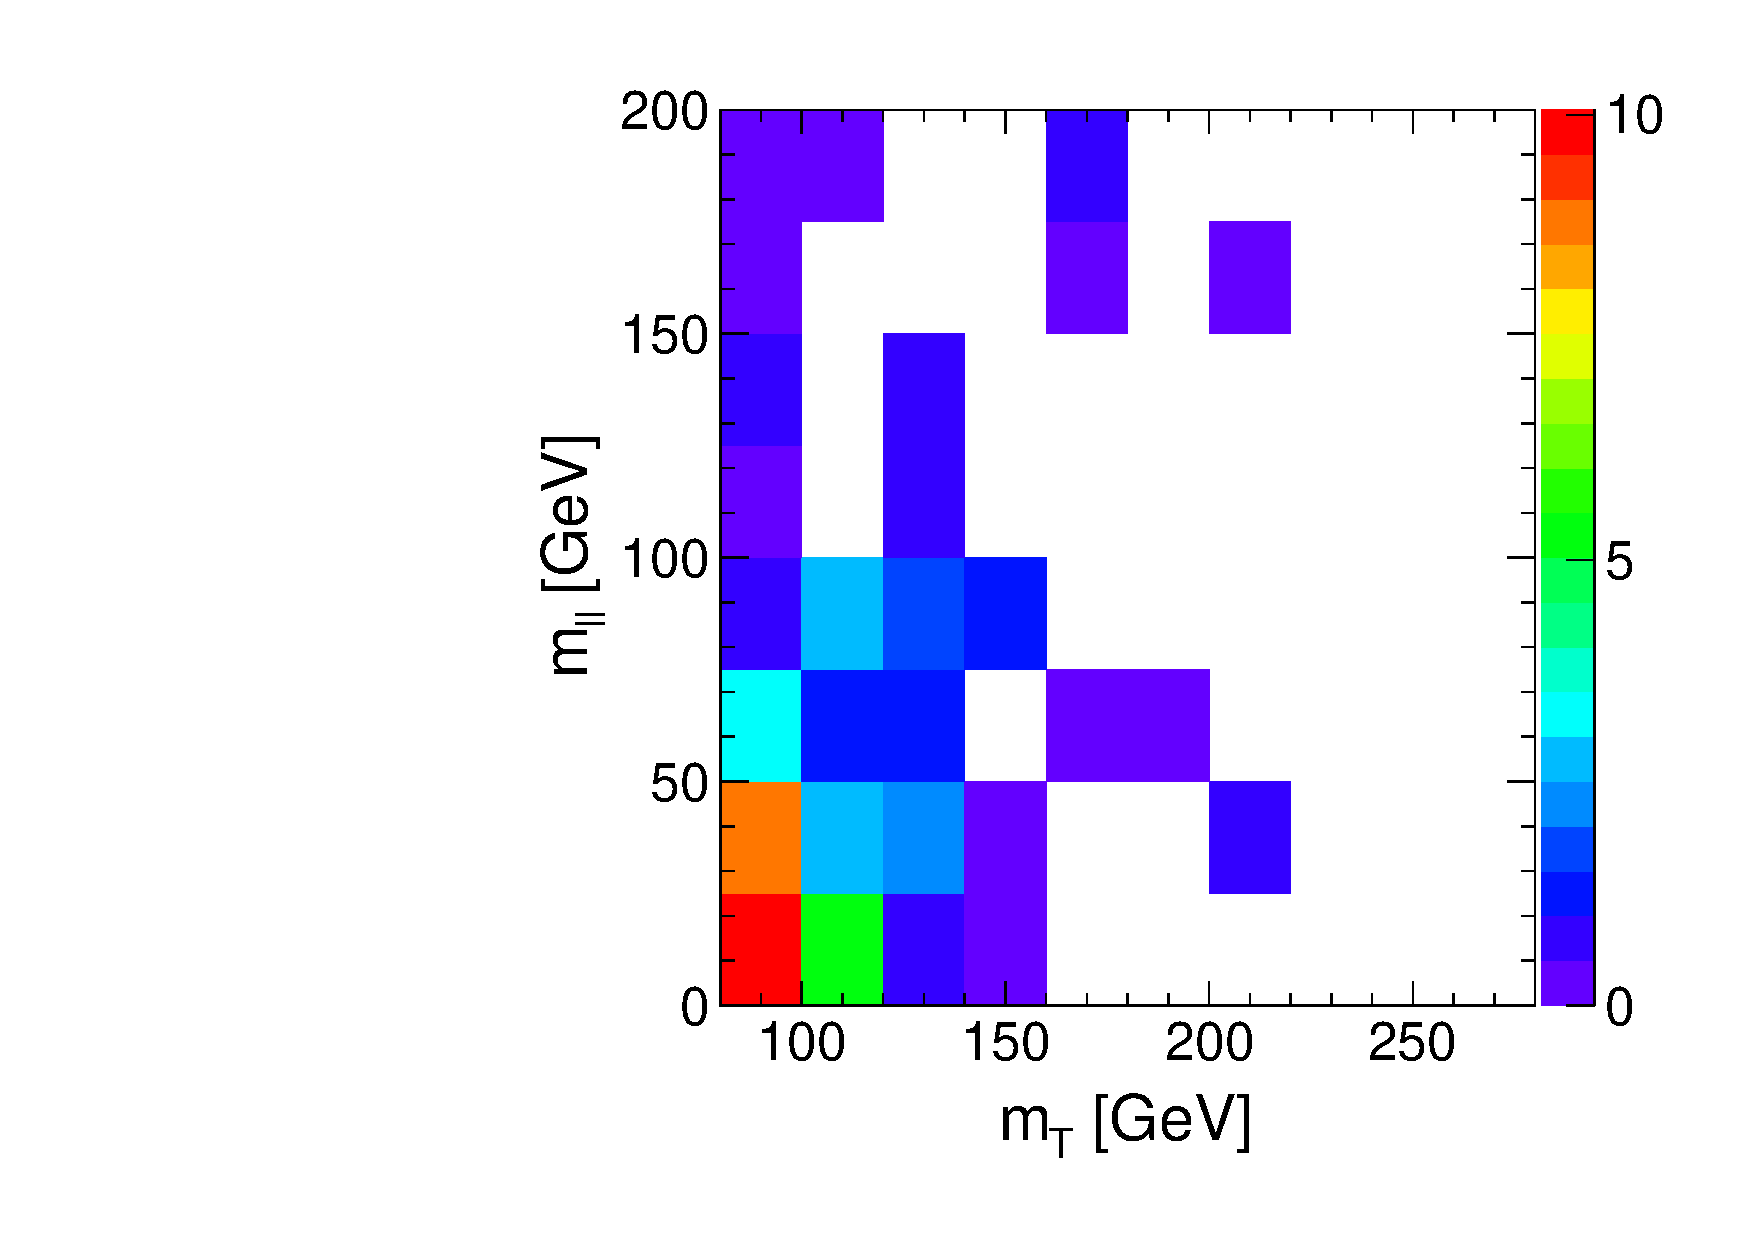
\includegraphics[width=.3\textwidth]{figures/mtvsmll_Wgamma_lowmass_0j.pdf}
} 
\caption{ The 2D ($m_{ll}, m_T$) templates for the main background processes in the 0-Jet with $m_H<300$ GeV.
}
\label{fig:bkg2d_lowmass_0j}
\end{figure}
%%%%%%%%%%%%%%%%%%%%%%%%%%%%%%%

%%%%%%%%%%%%%%%%%%%%%%%%%%%%%%%
\begin{figure}[!hbtp]
\centering
\subfigure[mH(300)]{
\centering
\label{subfig:h300_0j}
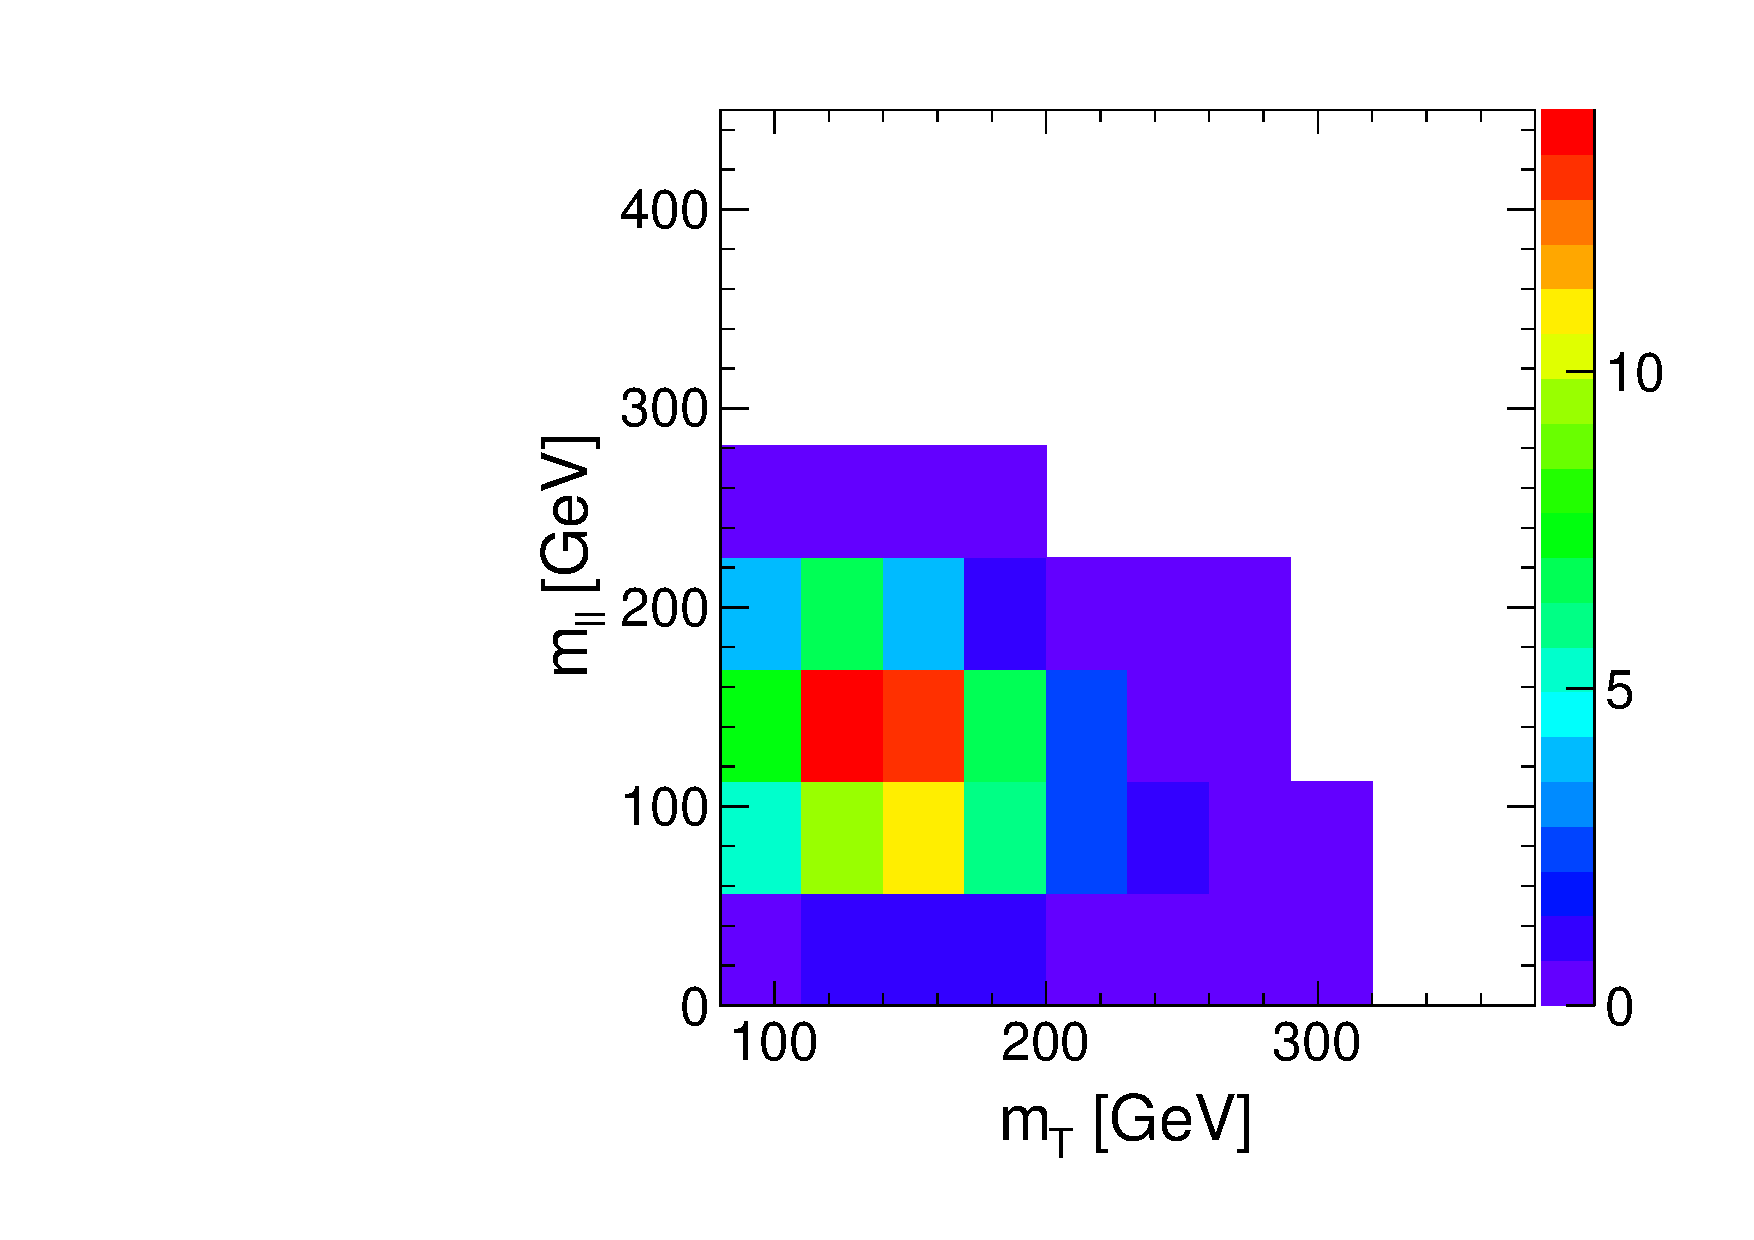
\includegraphics[width=.3\textwidth]{figures/mtvsmll_hww_300_0j.pdf}
}
\subfigure[mH(350)]{
\centering
\label{subfig:h350_0j}
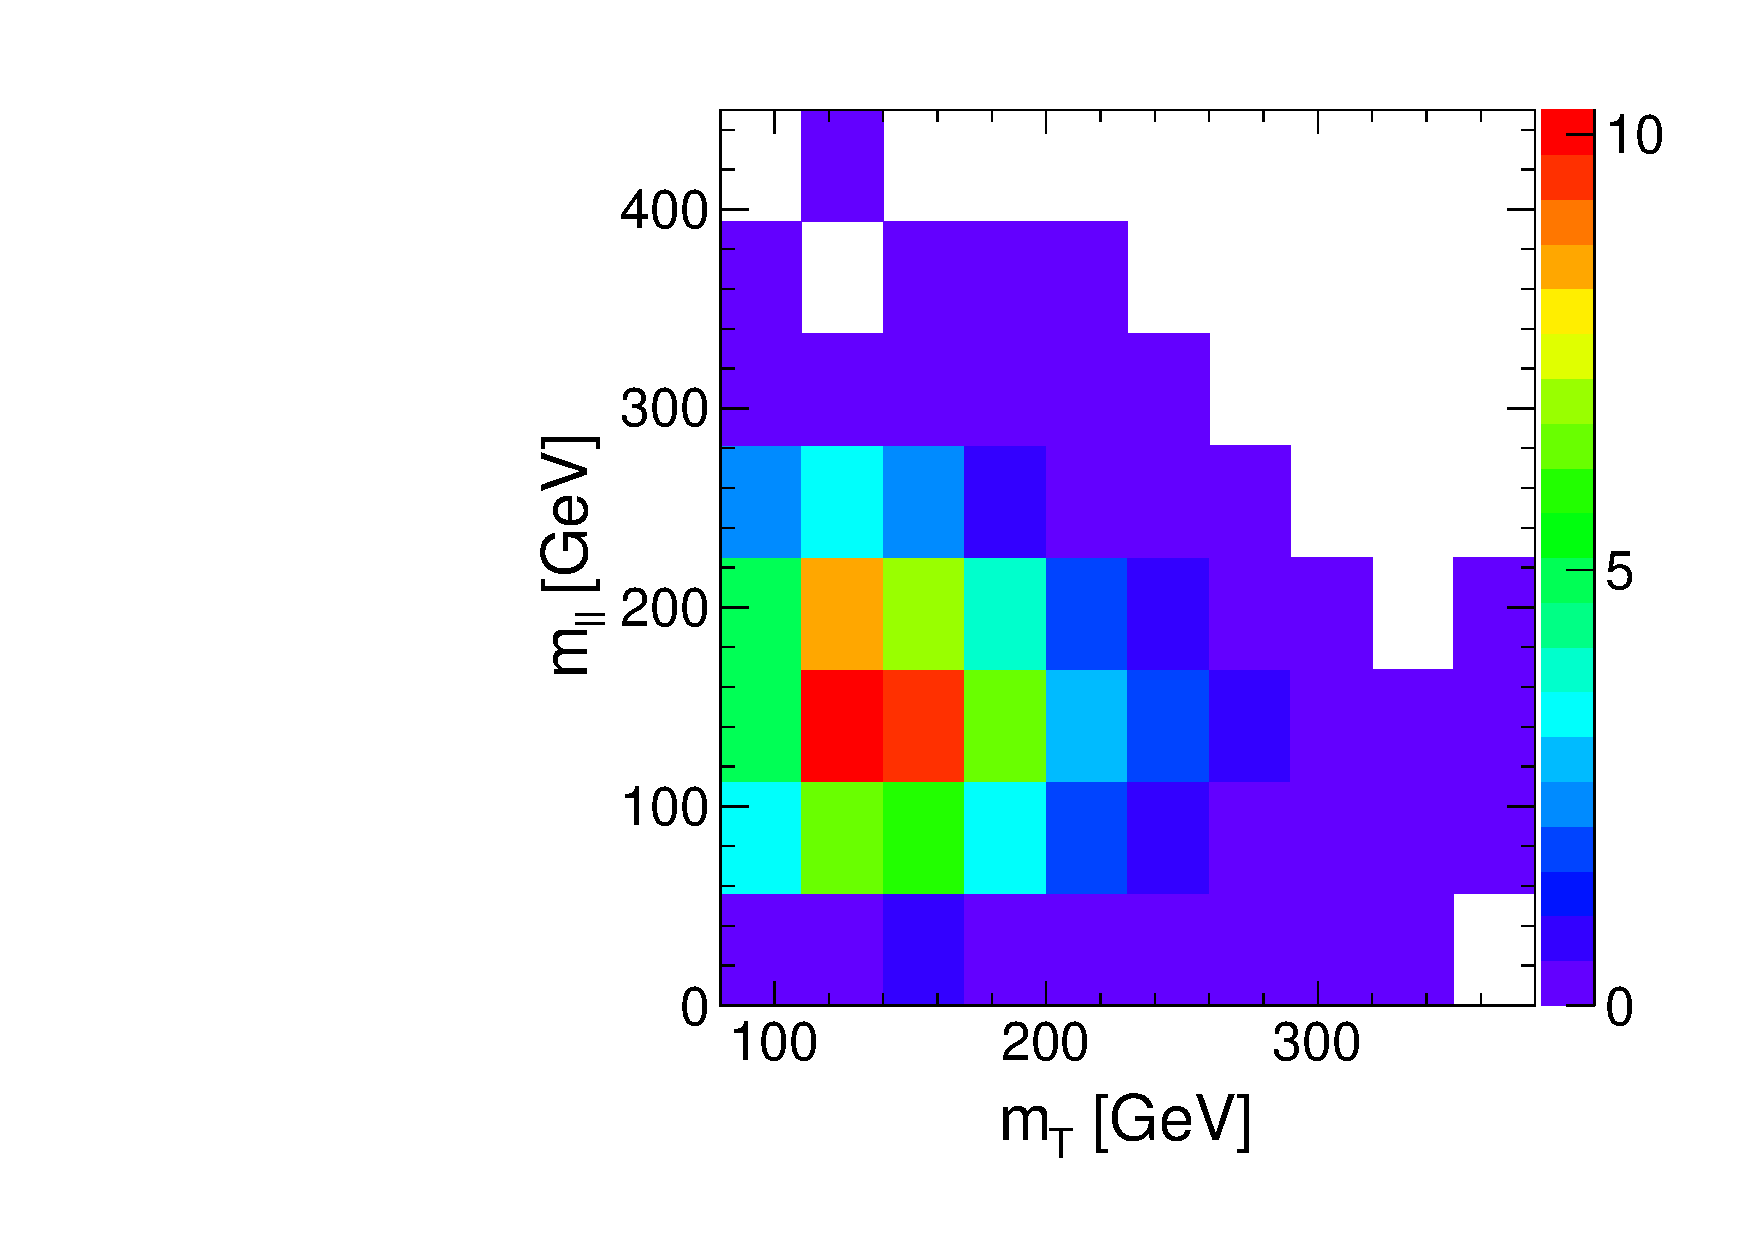
\includegraphics[width=.3\textwidth]{figures/mtvsmll_hww_350_0j.pdf}
} 
\subfigure[mH(400)]{
\centering
\label{subfig:h400_0j}
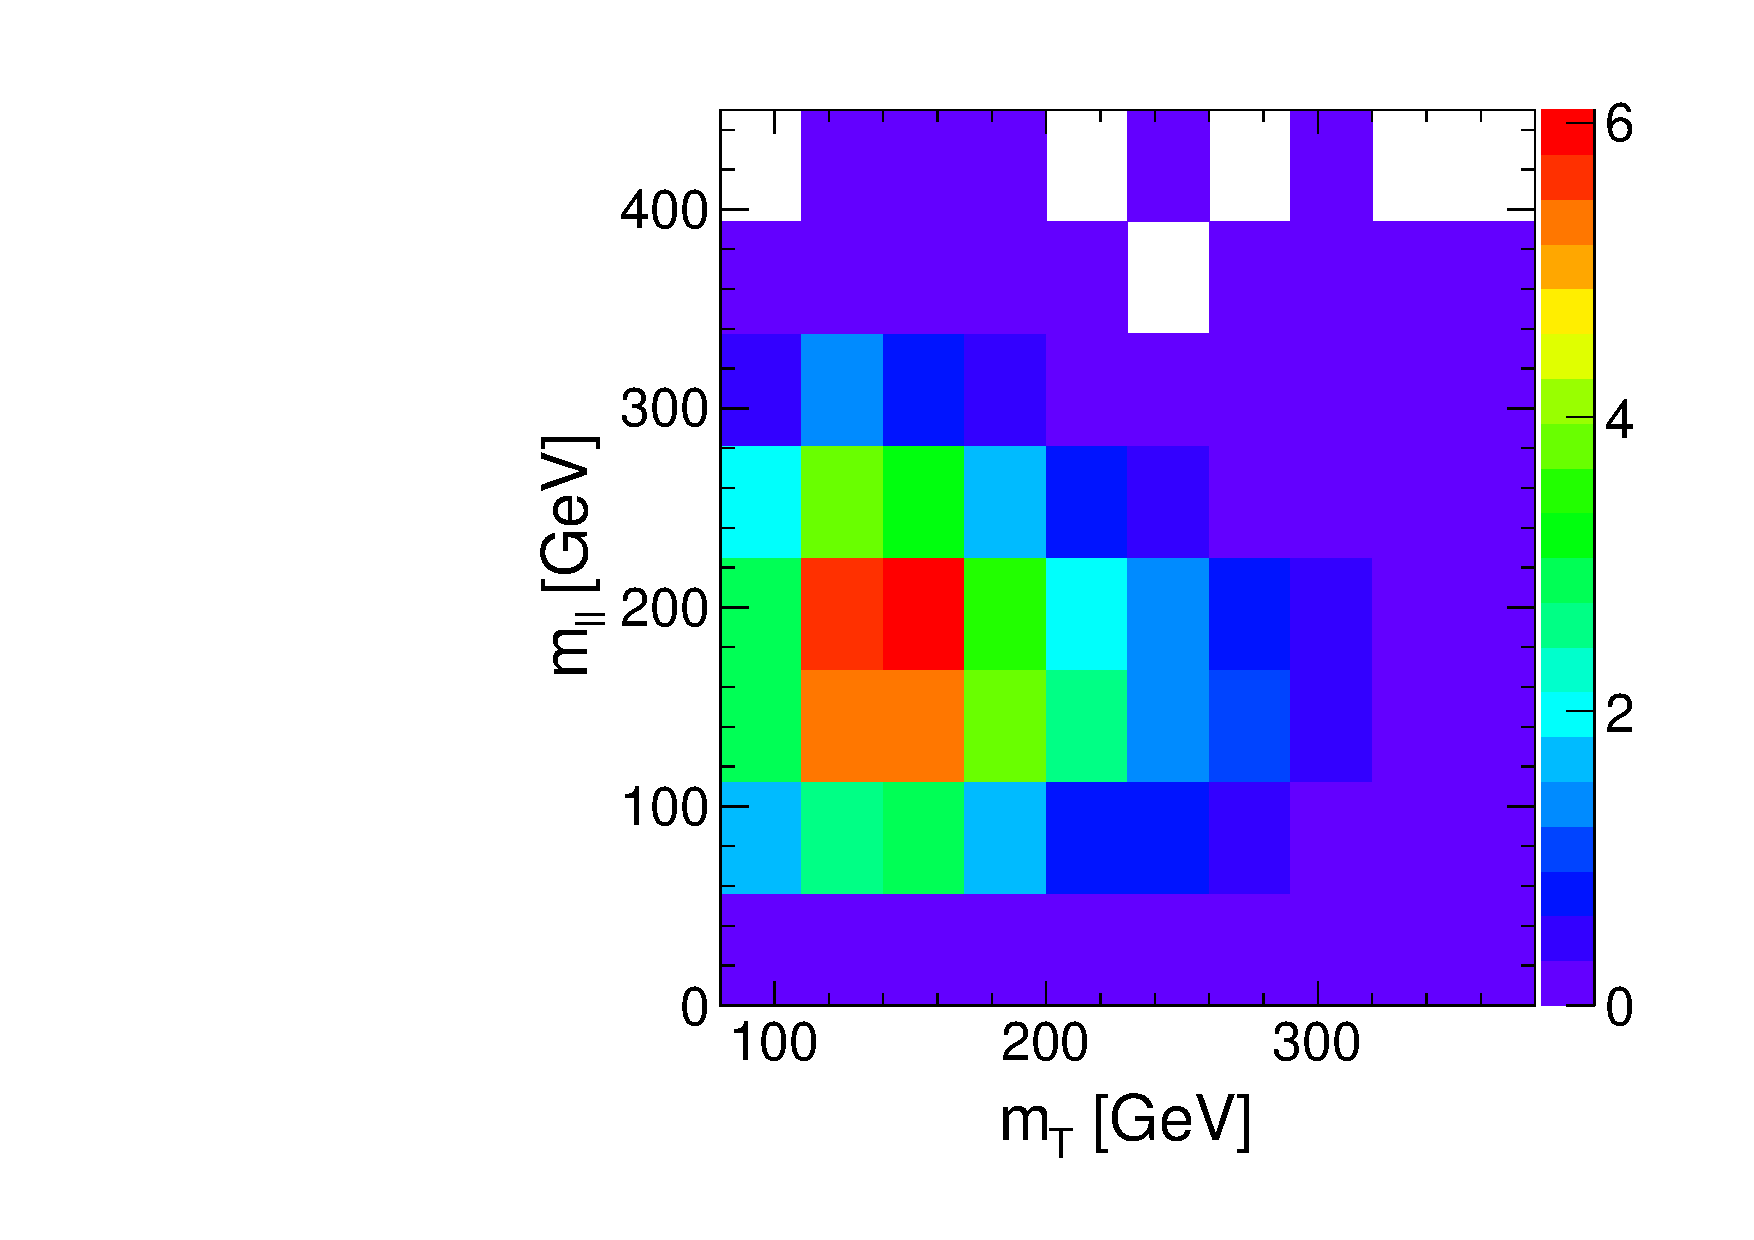
\includegraphics[width=.3\textwidth]{figures/mtvsmll_hww_400_0j.pdf}
}\\
\subfigure[mH(450)]{
\centering
\label{subfig:h450_0j}
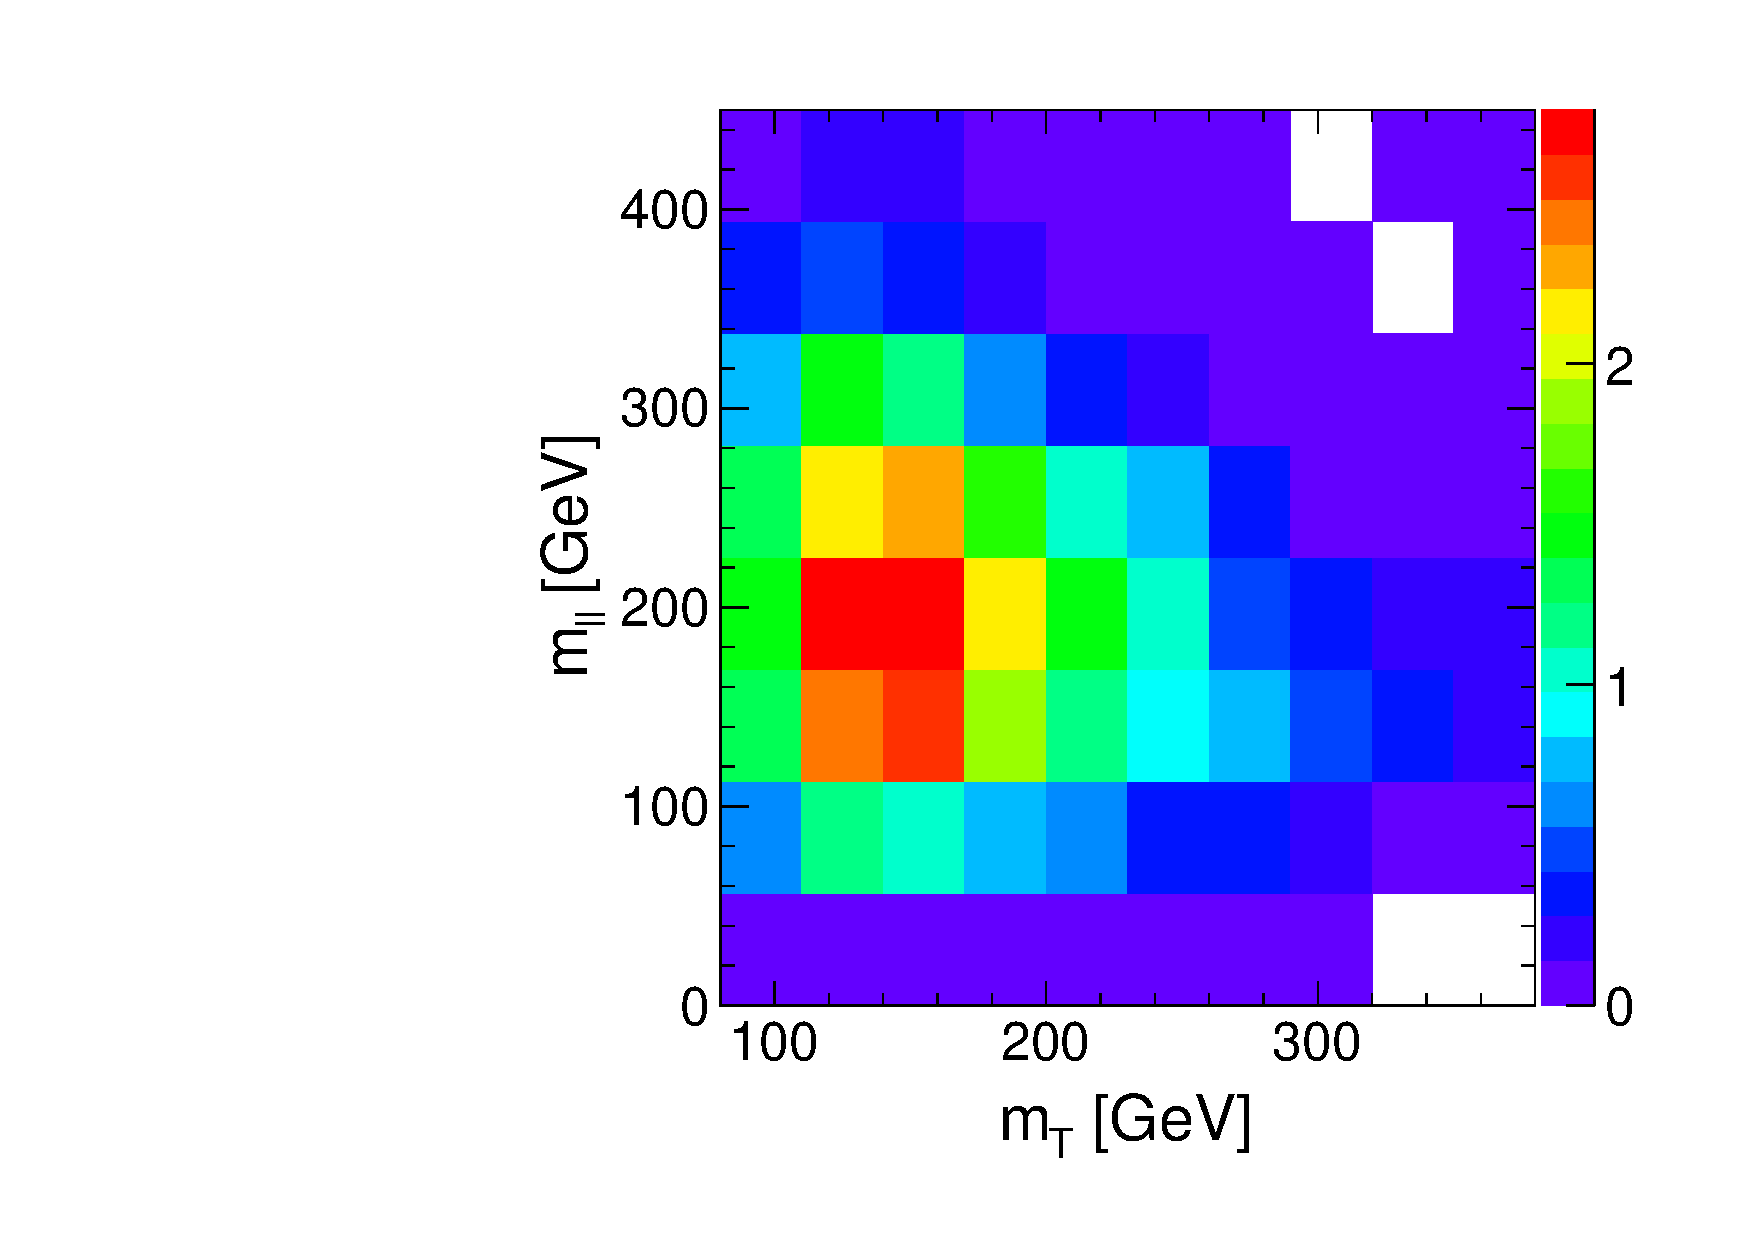
\includegraphics[width=.3\textwidth]{figures/mtvsmll_hww_450_0j.pdf}
}
\subfigure[mH(500)]{
\centering
\label{subfig:h140_0j}
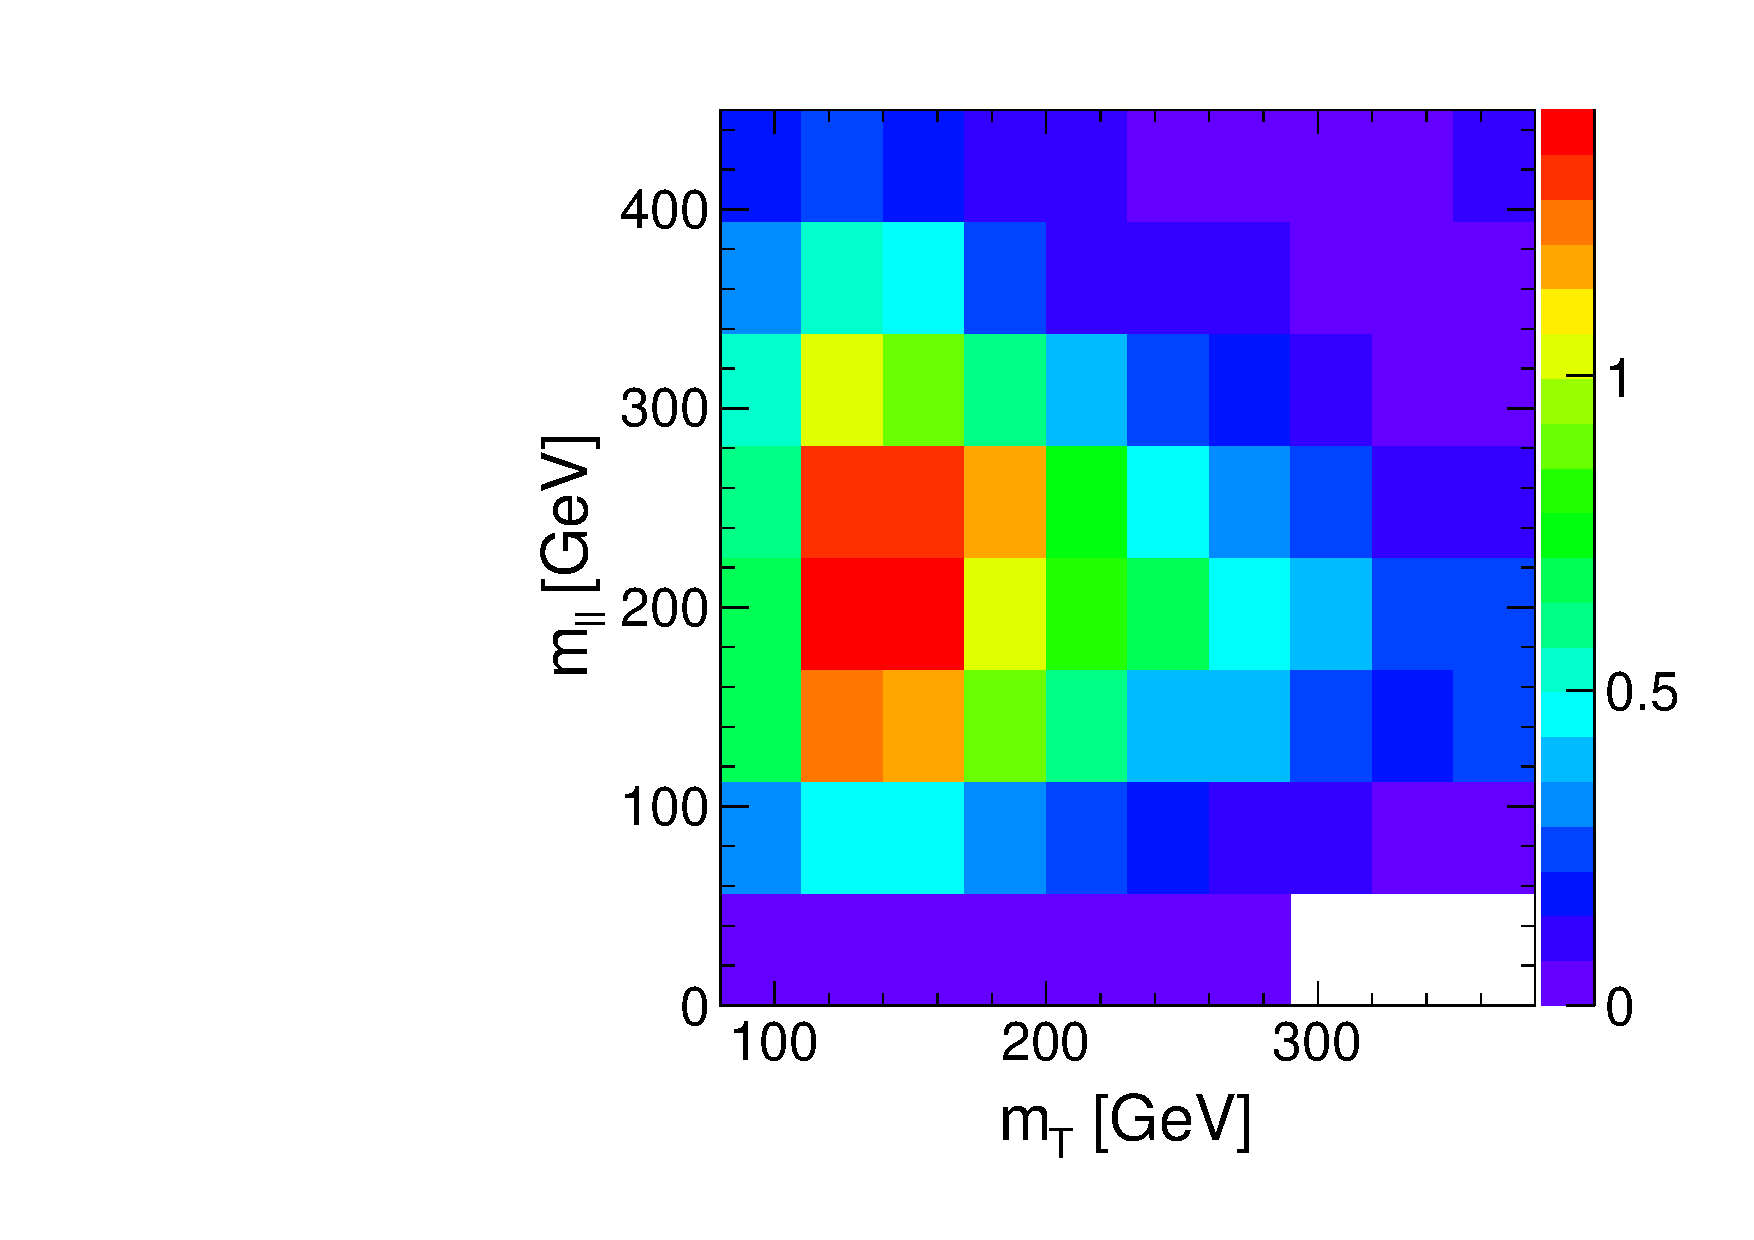
\includegraphics[width=.3\textwidth]{figures/mtvsmll_hww_500_0j.pdf}
}
\subfigure[mH(600)]{
\centering
\label{subfig:h150_0j}
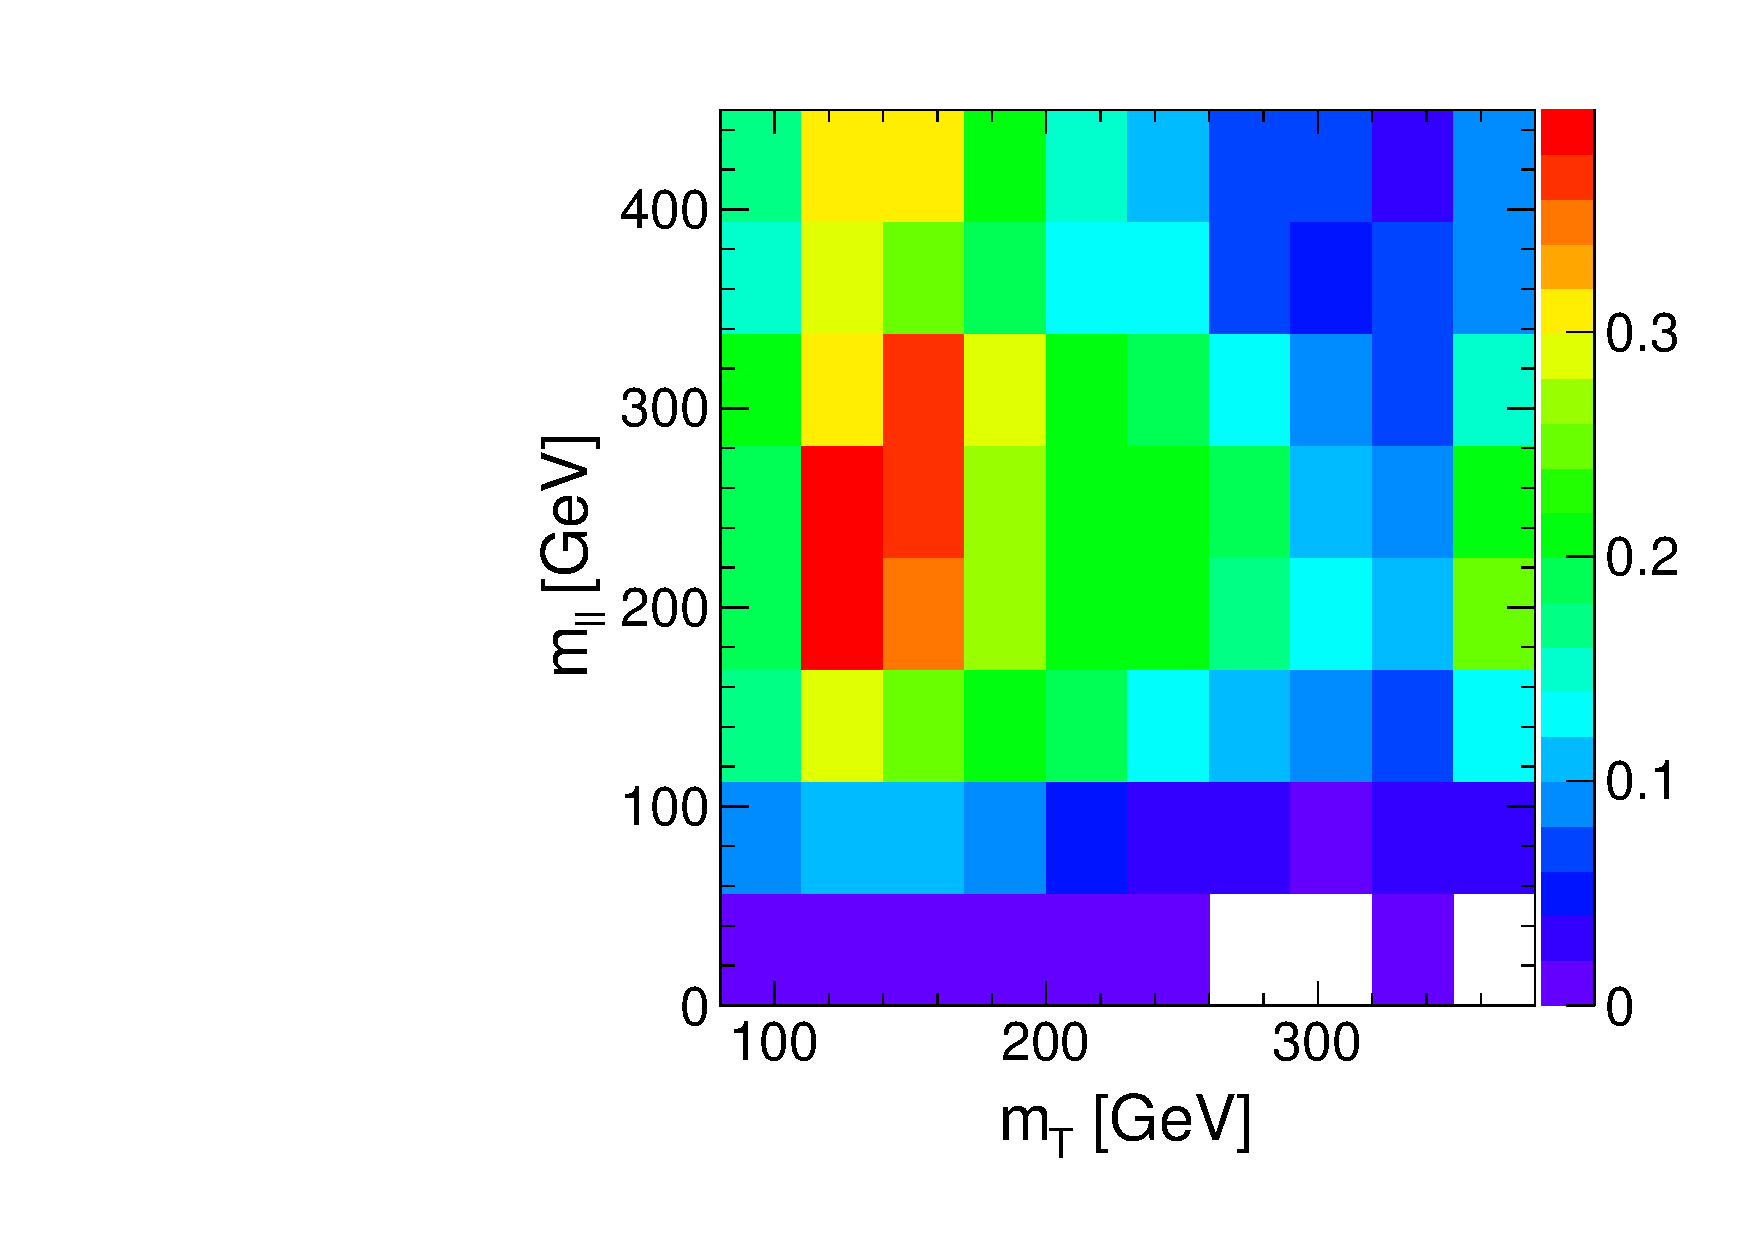
\includegraphics[width=.3\textwidth]{figures/mtvsmll_hww_600_0j.pdf}
} \\
\caption{ The 2D ($m_{ll}, m_T$) templates for the $gg\to H\to WW$ in the 0-Jet bin with $m_H>=300$ GeV. }
\label{fig:hww2d_highmass_0j}
\end{figure}
%%%%%%%%%%%%%%%%%%%%%%%%%%%%%%%


%%%%%%%%%%%%%%%%%%%%%%%%%%%%%%%
\begin{figure}[!hbtp]
\centering
\subfigure[$qq\to WW$]{
\centering
\label{subfig:qqww_0j}
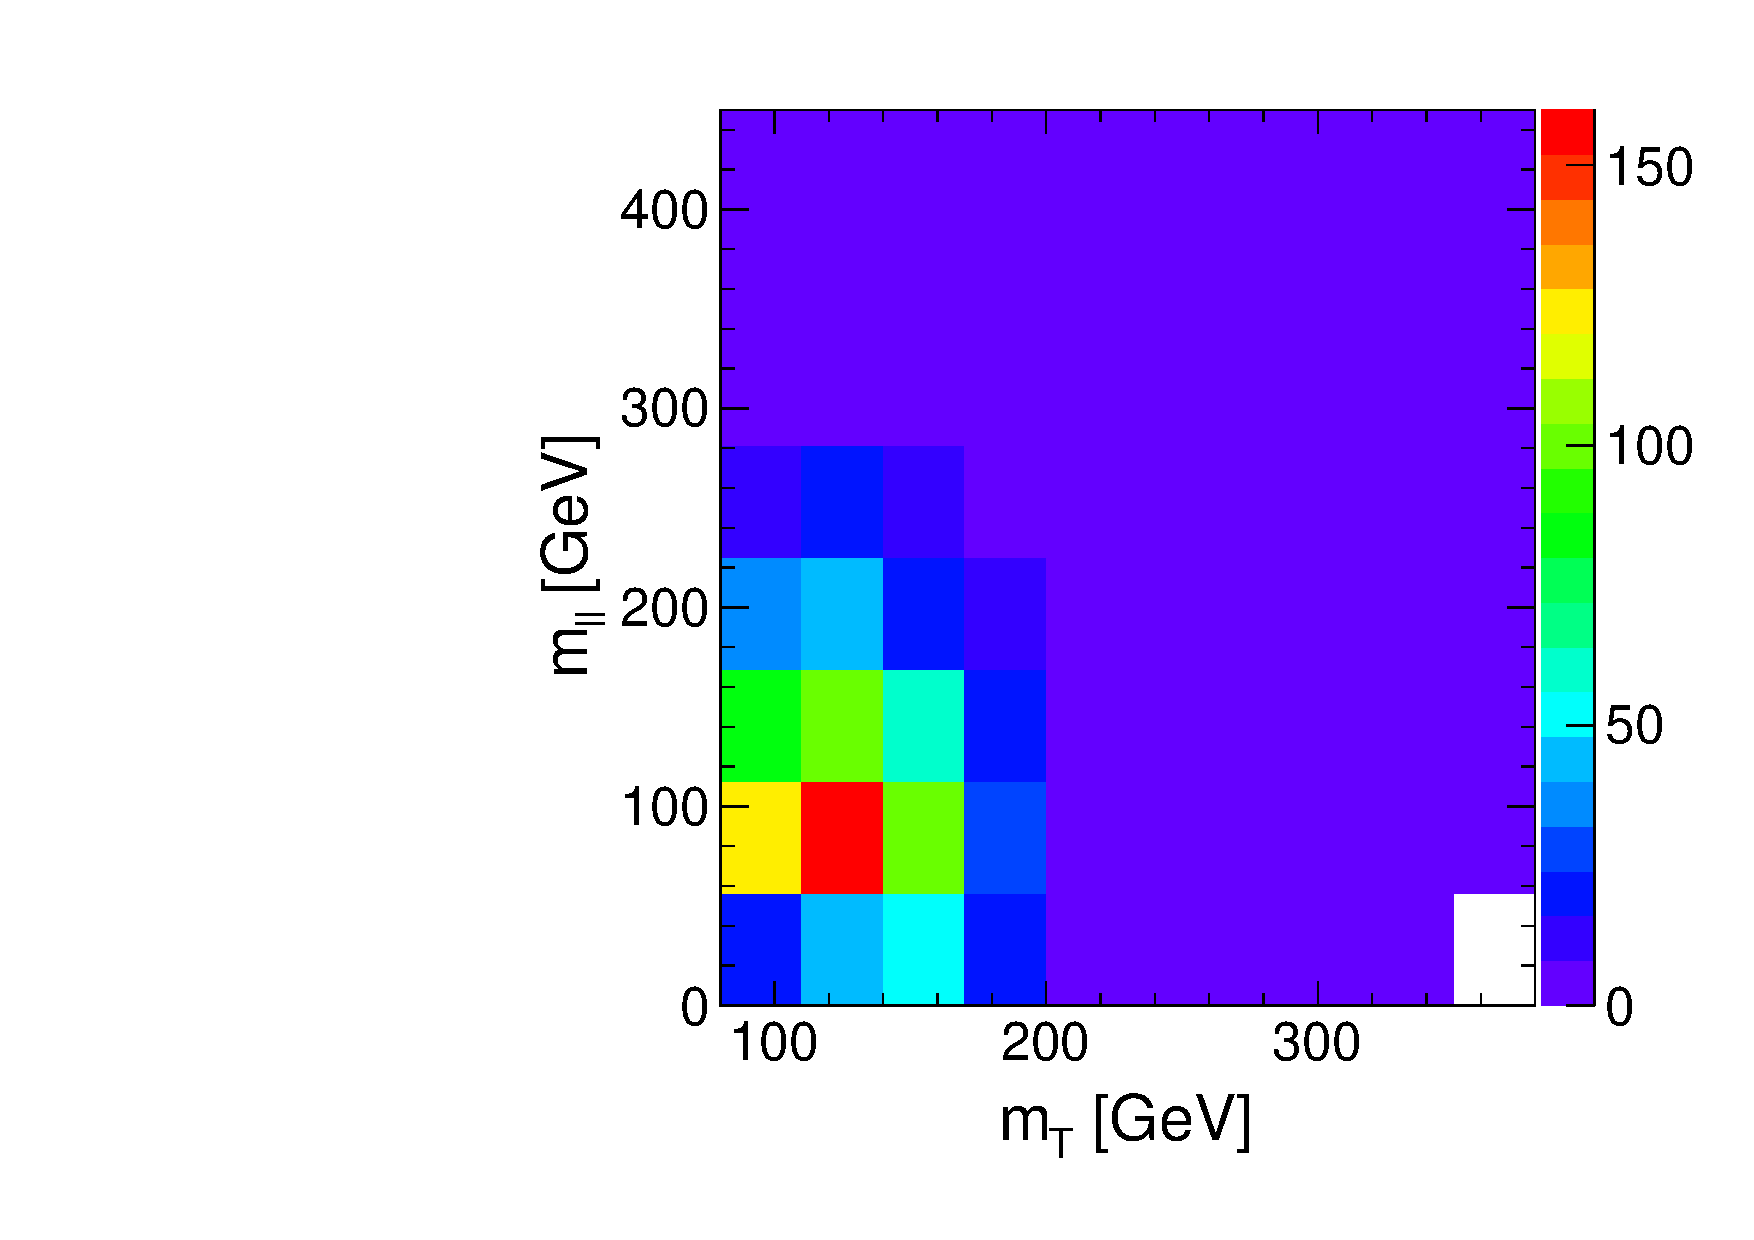
\includegraphics[width=.3\textwidth]{figures/mtvsmll_qqWW_highmass_0j.pdf}
}
\subfigure[Top]{
\centering
\label{subfig:top_0j}
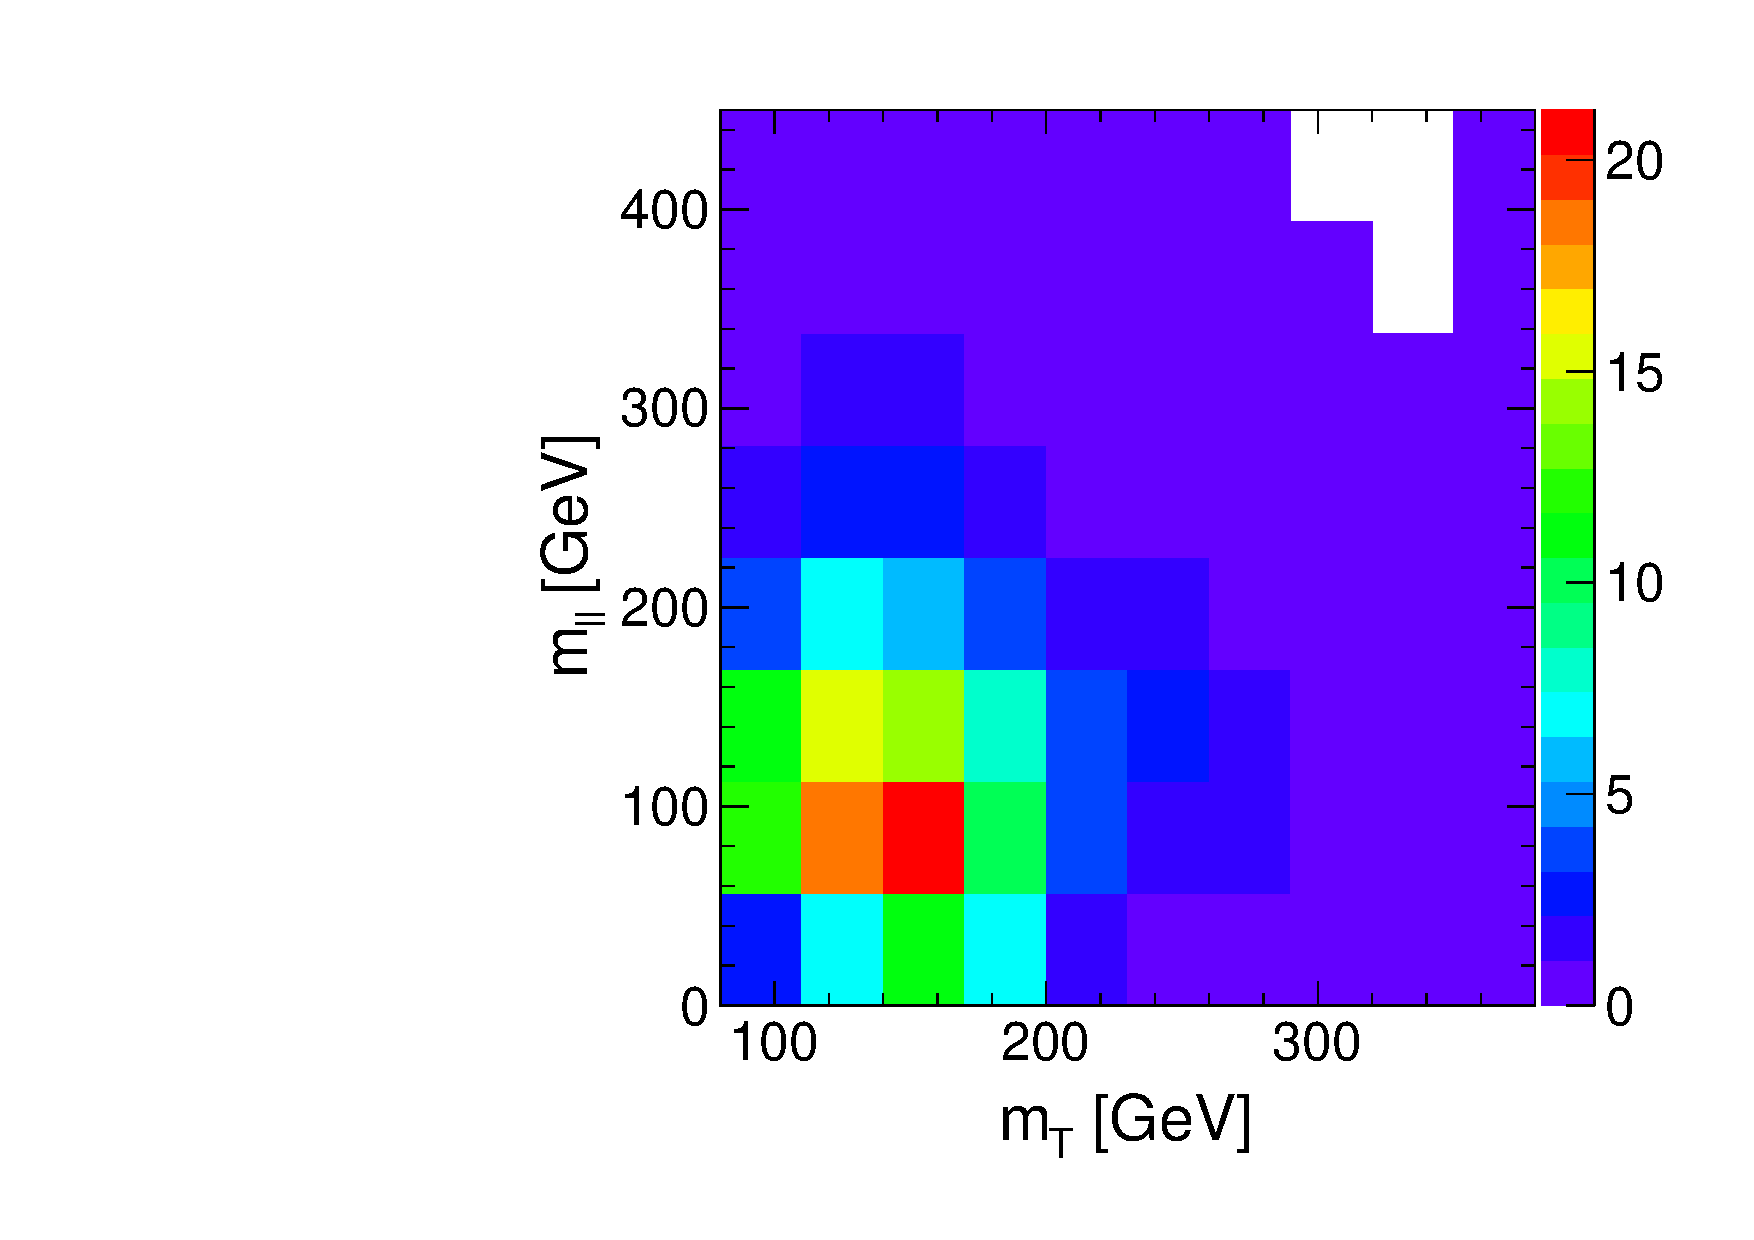
\includegraphics[width=.3\textwidth]{figures/mtvsmll_Top_highmass_0j.pdf}
} \\ 
\subfigure[Wjets]{
\centering
\label{subfig:wjets_0j}
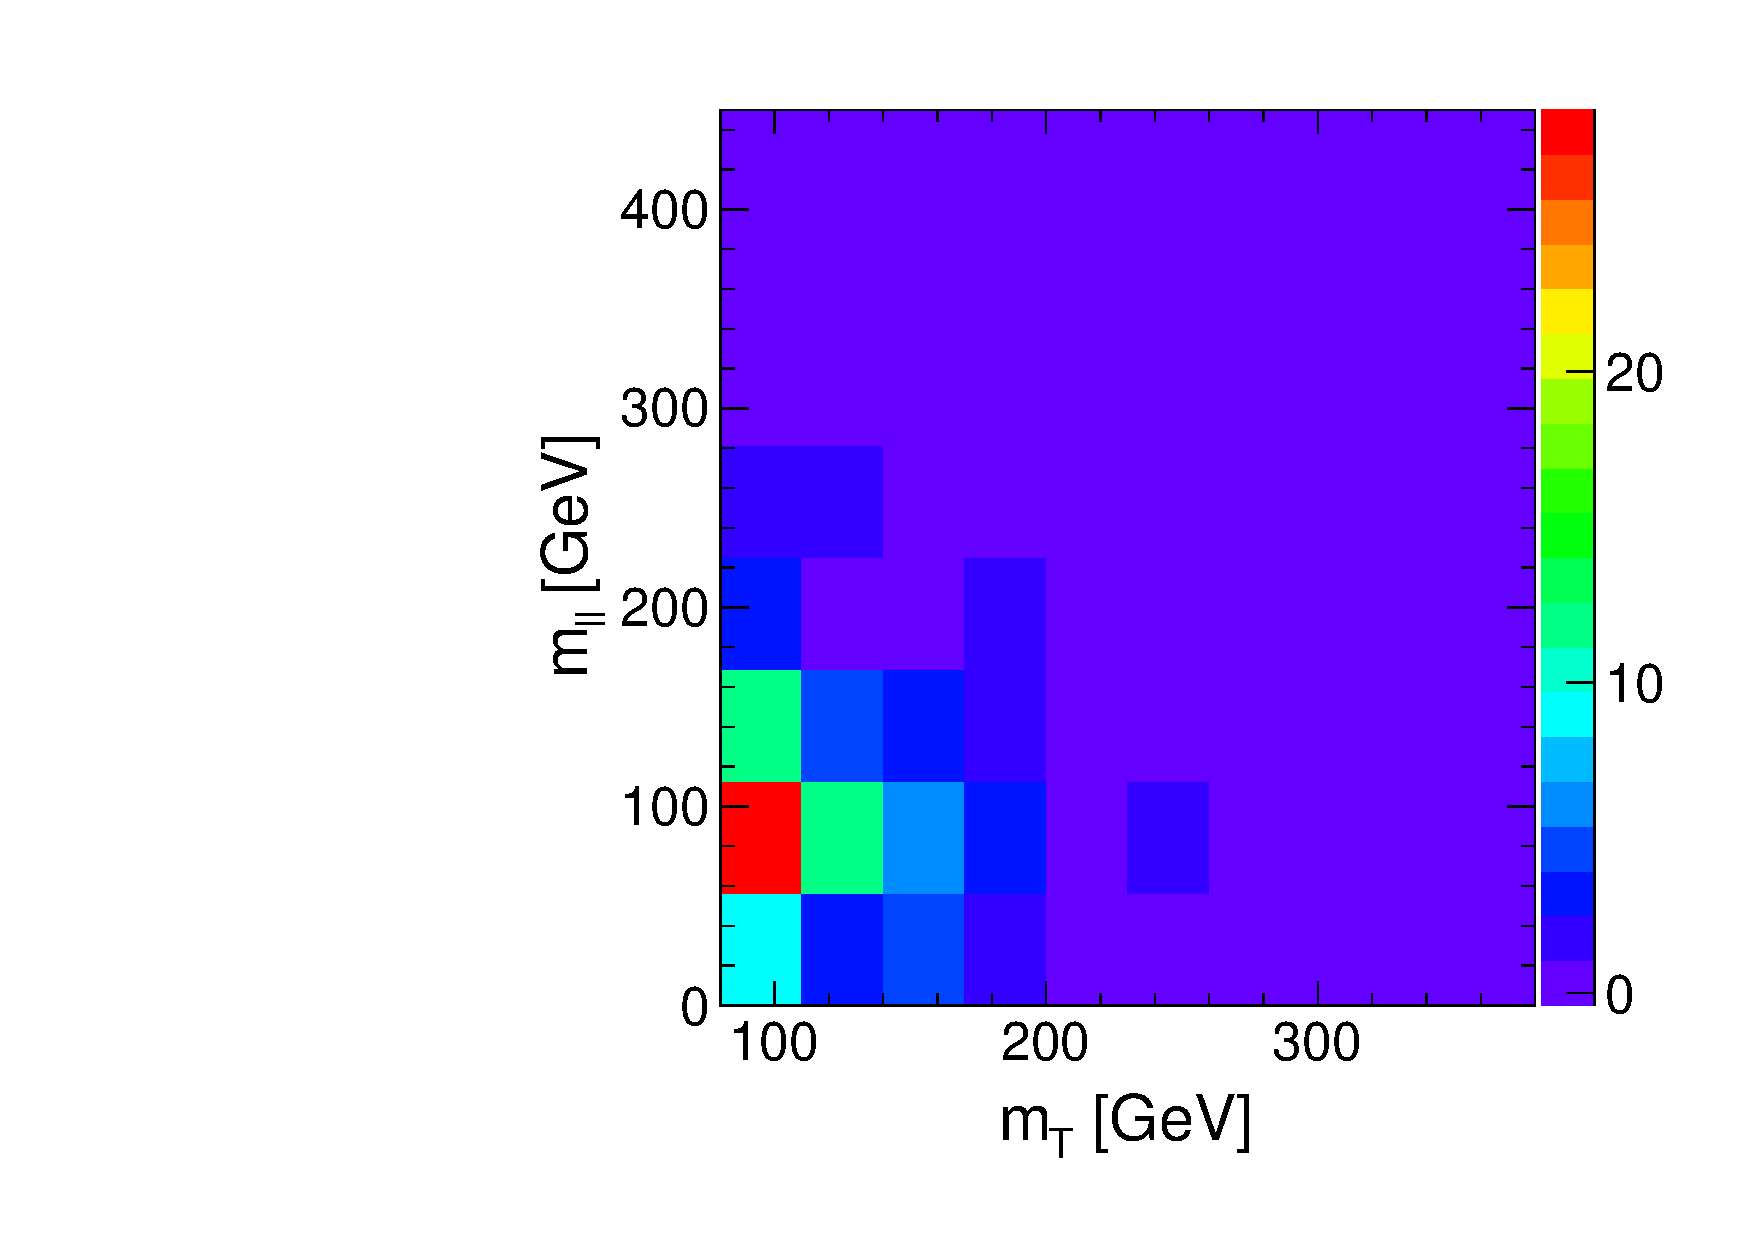
\includegraphics[width=.3\textwidth]{figures/mtvsmll_Wjets_highmass_0j.pdf}
}
\subfigure[$W\gamma$]{
\centering
\label{subfig:wgamma_0j}
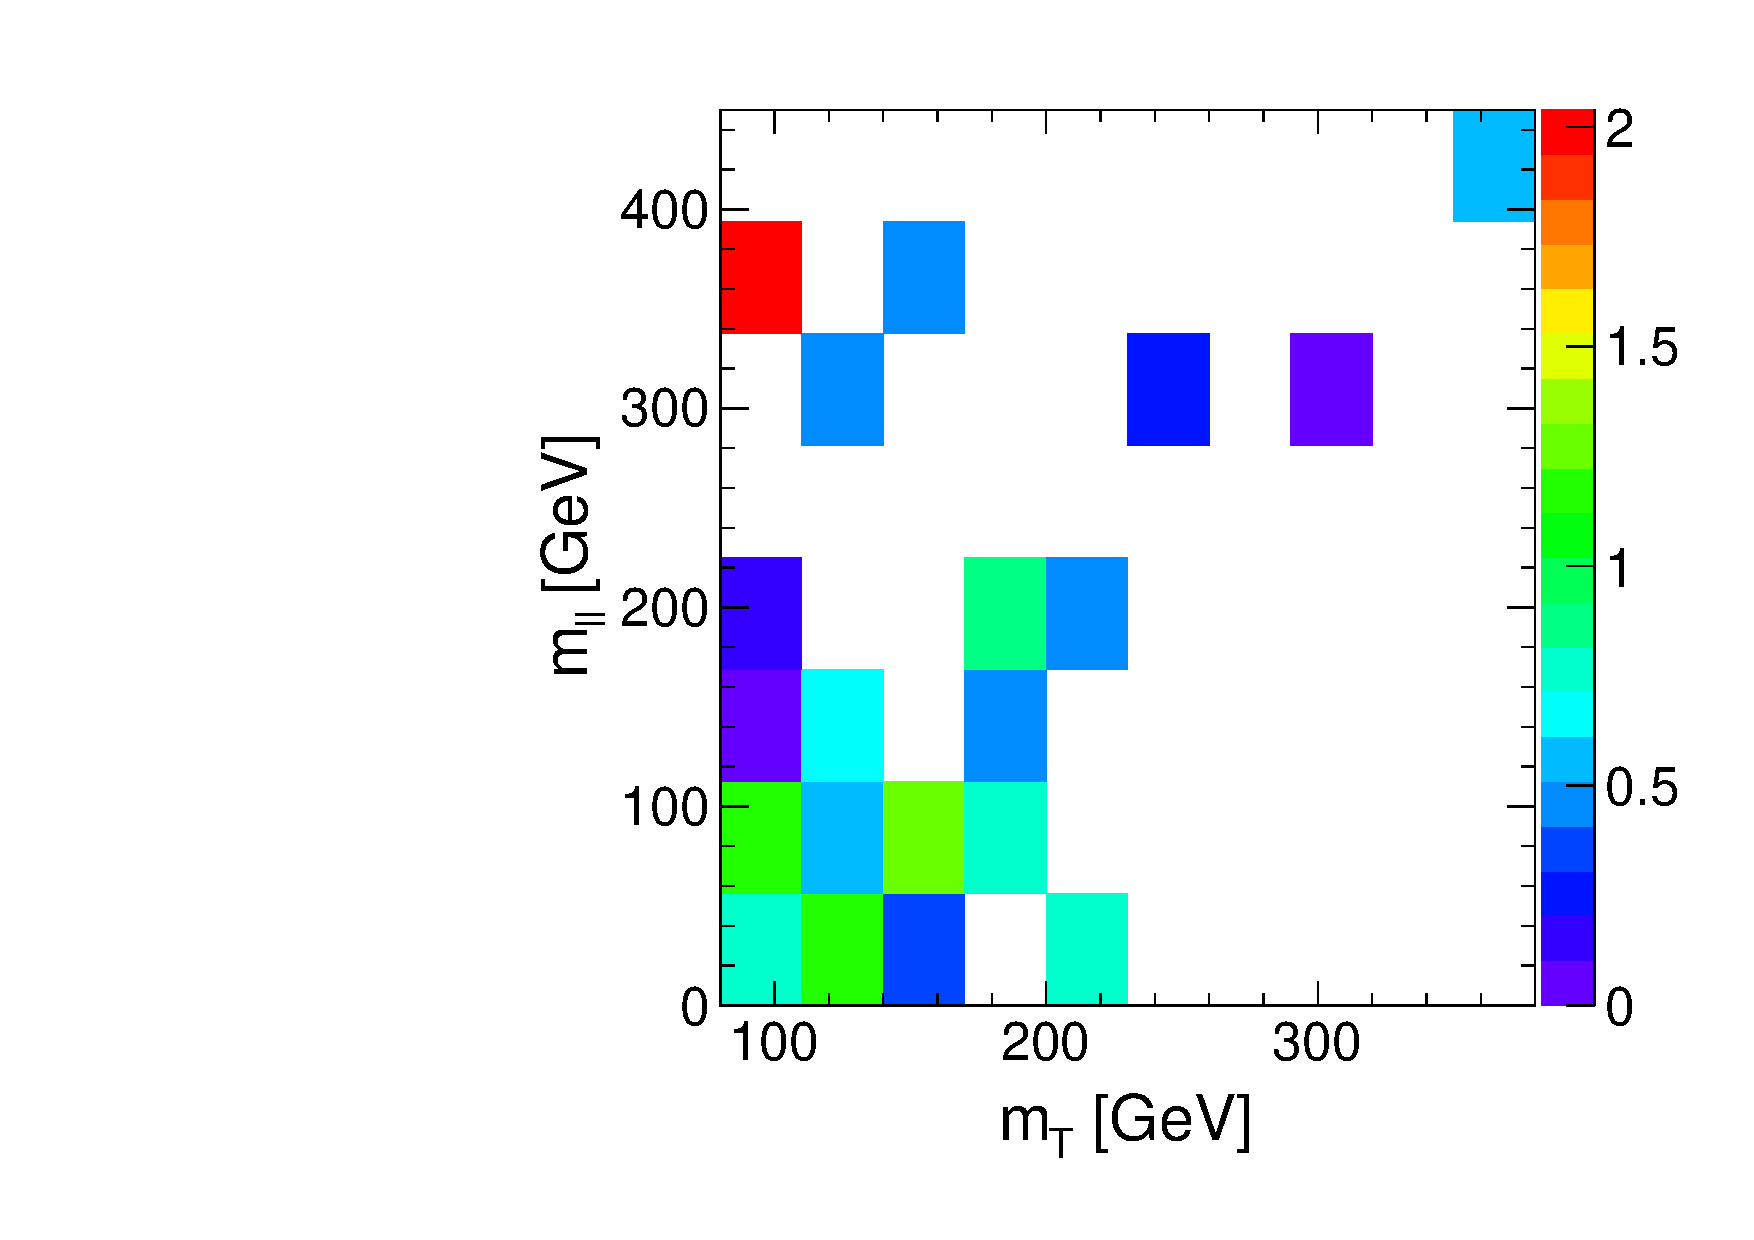
\includegraphics[width=.3\textwidth]{figures/mtvsmll_Wgamma_highmass_0j.pdf}
} 
\caption{ The 2D ($m_{ll}, m_T$) templates for the main background processes in the 0-Jet with $m_H>=300$ GeV.
}
\label{fig:bkg2d_highmass_0j}
\end{figure}
%%%%%%%%%%%%%%%%%%%%%%%%%%%%%%%


